\chapter{Modules}
\label{chap:Modules}

The source code of RespVis is structured into modules written in the ES module format.
Currently, all these modules are combined into a single, monolithic library bundle during the build process.
In the future, each module will be released on its own to allow users to import only the ones they need.
The reason for this is that most users will likely only require a subset of all the features included in the library, and it would unnecessarily increase the size of their bundles to import all of them.
A good example of this is D3, which also separates its considerable amount of features into different modules that can be successively added to a project when the need arises.

At the time of writing, the RespVis library contains five different modules: the Core, Legend, Tooltip, Bar, and Point Modules.
Each of these modules contains submodules that have been grouped by thematic similarity.
The Core Module holds the core functionality of the library that all other modules depend on and includes the Layouter and Axis Components, Chart and Chart Window base functionality, and various utility functions and types.
The Legend Module contains the implementation of a Legend Component that is mostly meant to describe discrete data by rendering distinct values as labeled symbols.
The Tooltip Module holds functions to control the showing, placement, and content of Tooltips, as well as utility functions that simplify the configuration and initialization of Tooltips on Series Components.
The Bar Module distinguishes between Single-Series, Grouped, and Stacked Bars and includes various low-level and high-level components to render each of those types.
Similarly, the Point Module contains low-level and high-level components to visualize Point Charts.
All of the different modules and the dependencies between them are shown in Figure~\ref{fig:Modules}.

\begin{figure}[tp]
\centering
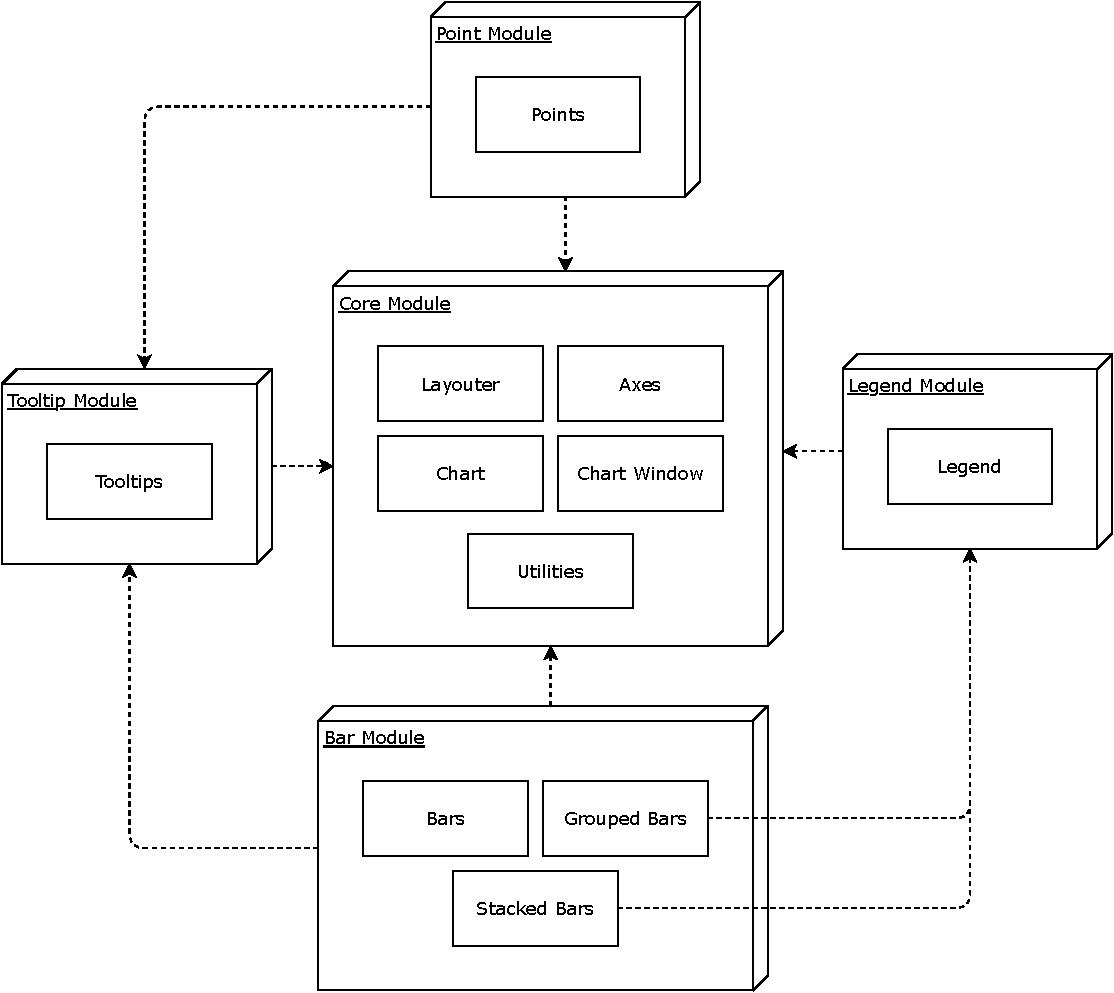
\includegraphics[keepaspectratio,width=\linewidth,height=\fullh]{diagrams/respvis-modules.pdf}
\caption[Modules of RespVis]{
  This diagram shows the different modules of the RespVis library.
  It also shows the most important submodules contained in the individual modules.
  The directional arrows connecting modules indicate dependencies between them.
  \imgcredit{Image created by the author of this thesis using \href{https://www.diagrams.net/}{diagrams.net}.}
}
\label{fig:Modules}
\end{figure}


\section{Core Module}

The Core Module contains the necessary core functionality of the library.
It is the base module that all other modules depend on and includes various utility functions, the Layouter, Axes, Chart base functionality, and Chart Window base functionality.
RespVis heavily relies on utility functions to reuse and structure recurring operations.
The Core Module contains utilities to deal with arrays, elements, Selections, and texts, as well as geometric utilities that simplify the handling of positions, sizes, rectangles, circles, and paths.
The Layouter is a custom component that enables controlling the layout of SVG elements with CSS.
Axis Components have been included in the Core Module because they are important components that occur in nearly every visualization.
Lastly, the Core Module offers Chart and Chart Window base functionalities that simplify the creation of more specialized Charts and Chart Windows.
The implementation of the Core Module is located in the \code{src/lib/core/} directory of the project.

\subsection{Utilities}

The utilities provided by RespVis are split into multiple modules that are placed in the \code{utilities/} directory of the core module.
These modules include types and functions that perform array, element, Selection, and text operations, as well as modules that simplify geometric operations with positions, sizes, rectangles, circles, and paths.
Utility functions are grouped into modules by the type of entity on which they operate.
This grouping is also reflected in the names of functions because they all begin with the type of entity with which a function is associated.

Array utilities can be found in the \code{utilities/array.ts} module.
The \code{Array} class in the JavaScript base implementation already offers a wide variety of convenient methods to work with arrays.
These methods form a solid foundation to handle a broad range of situations, but not everything is covered, and some things require manual implementations, which is why the RespVis library offers additional functions that simplify commonly encountered tasks.
The \code{arrayEquals} function is used to verify the equality of two arrays and also works if they contain nested arrays within them.
Type guard functions are used to determine the type of a variable at runtime.
For this purpose, two different array type guard functions are provided in the array utility module: \code{arrayIs}, which evaluates to true if the passed parameter is an array, and \code{arrayIs2D}, which evaluates to true if the handed parameter is a two-dimensional array.
The \code{arrayIs} function is merely a wrapper around the \code{Array.isArray} method.
Theoretically, the \code{Array.isArray} method could be used directly instead of the \code{arrayIs} function, but because the \code{arrayIs2D} function is required, the \code{arrayIs} function has also been added for consistency reasons.
The last function in the array utility module is the \code{arrayPartition} function.
This function receives an array and a partition size as parameters and returns a partitioned version of the input array with each chunk containing the number of items specified by the partition size parameter.


The Element Utility Module located at \code{utilities/elements.ts} in the Core Module contains functions and constants related to elements in a document.
The \code{elementRelativeBounds} function is used to calculate the bounding box of an element relative to the bounding box of its parent in viewport coordinates.
Internally, it uses the \code{getBoundingClientRect} function, which returns the actual bounding box of an element in viewport coordinates and, as opposed to other ways of accessing an element's position, it also takes transformations into account.
Every element has a set of CSS styles applied to them, and the \code{Window.getComputedStyle} method can be used to access the active style of an element.
The style declaration object returned by this method contains all possible CSS properties and their values, regardless of whether or not they are set to default values.
Sometimes this behavior may be desired, but in this library, the computed style is used to prepare a downloadable SVG document to transform styling information set in CSS to attributes on the individual elements.
If every possible CSS property on every element would be mapped to an attribute, the resulting SVG document would be unnecessarily bloated because only those properties that are not set to their default values actually have an effect.
For this reason, the \code{elementComputedStyleWithoutDefaults} function has been implemented to calculate the computed style of an element and remove all properties that are at default values from the returned style declaration object.
This is implemented by adding a \code{<style-dummy>} element as a sibling of the element of interest, getting the computed styles of both elements, and calculating the difference between them.
To accelerate these calculations, the \code{elementComputedStyleWithoutDefaults} function accepts an array of property names as its second parameter and will only consider the properties listed in this array.
The constant \code{elementSVGPresentationAttrs} array contains all names of the presentation attributes listed in the SVG 1.1 specification \parencite{SVG11}.
Since only these SVG attributes can be styled via CSS, only these properties must be considered when preparing downloadable SVG documents.

Selection utilities are implemented in the \code{utilities/selection.ts} module.
They include typing improvements for the D3 \code{Selection}, \code{Transition}, and \code{SelectionOrTransition} interfaces and type guards to distinguish between Selections and Transitions.
The \code{Selection}, \code{Transition}, and \code{SelectionOrTransition} interfaces allow the specification of four type variables: the type of elements contained in the Selection or Transition, the type of data bound to those elements, the type of the parents of those elements, and the type of data bound to those parents.
In most cases, the type variables related to parent elements do not influence the logic of code using these interfaces and could be omitted to keep it more concise.
For this reason, these interfaces have been reexported with default types set on all of the type variables, which means that whenever type variables need to be manually specified, only those that need to be set to specific types need to be explicitly stated.
Further typing improvements have been made to the \code{attr} and \code{dispatch} methods of the \code{Selection} interface.
The D3 type declarations of the \code{Selection.attr} method do not include \code{null} as a possible return value, which is wrong because this method will result in a \code{null} value when reading an attribute that does not exist.
To fix this inconsistency and catch potential bugs related to it during compilation, the type declaration of the \code{Selection.attr} method has been overwritten in the Selection Utility Module to include \code{null} as a possible return value.
A less important but convenient improvement has been made to the type declaration of the \code{Selection.dispatch} method.
This method allows the dispatching of custom events with certain parameters that control different aspects of how this event is dispatched and the data bound to it.
In practice, not all parameters need to be specified at every invocation because the implementation of the \code{Selection.dispatch} method will provide default values for all of them, but this is not reflected in the type declaration of the function, which requires every parameter to be set every time the function is called.
To fix this, the Selection Utility Module provides a type declaration overwrite for the \code{Selection.dispatch} function that wraps the type of the parameters parameter into the \code{Partial} utility type.
Apart from these typing improvements, this module also provides the \code{isSelection} and \code{isTransition} type guard functions that are used to distiguish between Selections and Transitions.


Utilities for dealing with \code{<text>} elements can be found in the \code{utilities/text.ts} module.
It contains rather basic functionalities that simply set specific \code{data-*} attributes to specific values on \code{<text>} elements.
The Text Utility Module holds functions that set \code{data-*} attributes controlling the horizontal and vertical alignment of \code{<text>} elements, as well as their orientation.
Horizontal and vertical alignment is configured using the \code{textAlignHorizontal} and \code{textAlignVertical} functions.
These functions respectively set the \code{data-align-h} and \code{data-align-v} attribute on a Selection or Transition to the value passed into either function as a string enum parameter of type \code{HorizontalAlignment} or \code{VerticalAlignment}.
The \code{HorizontalAlignment} enum represents the string values \code{\"left\"}, \code{\"center\"} and \code{\"right\"}, while the \code{VerticalAlignment} enum represents the values \code{\"top\"}, \code{\"center\"} and \code{\"bottom\"}.
The distinct \code{data-align-h} and \code{data-align-v} attribute values are then used in the Selectors of CSS rules to declare different \code{text-anchor} and \code{dominant-baseline} property values.
Text orientation is set using the \code{textOrientation} function, which sets the \code{data-orientation} attribute on a Selection or Transition to the value specified via the string enum parameter of type \code{Orientation}.
The \code{Orientation} enum represents the values \code{\"horizontal\"} and \code{\"vertical\"}.
These \code{data-orientation} attribute values are then used in CSS to set the \code{text-anchor}, \code{dominant-baseline}, and \code{transform} properties of a \code{<text>} element, in order to rotate it accordingly and position it correctly inside the bounding box calculated by the layouter.


The Core Module also contains utilities that simplify geometric operations.
One of these utilities is the Position Utility Module located in the \code{utilities/position.ts} file.
This module contains the \code{Position} interface and various functions to perform operations related to it.
The \code{Position} interface consists of the \code{x} and \code{y} number properties.
Rounding these properties is necessary to be able to correctly compare the equality of two \code{Position} objects and to not render unnecessarily long strings when transforming them into string representations.
This rounding is performed with the \code{positionRound} function, which allows the specification of the number of decimals the properties should be rounded on.
Equality comparision between two \code{Position} objects can be done with the \code{positionEquals} function, which evaluates to \code{true} if both \code{Position} objects are equal and \code{false} if not.
To transform a \code{Position} object into its string representation of the form \code{\"x, y\"}, the \code{positionToString} function can be used.
Its counterpart, the \code{positionFromString} function, can be used to transform a string of the correct format into a \code{Position}.
A large part of RespVis consists of modifying the attributes of elements.
Therefore, the \code{positionToAttrs} function can be used to set the \code{x} and \code{y} attributes of a \code{SelectionOrTransition} to the values of the \code{x} and \code{y} members of a \code{Position}.
Similarly, the \code{positionToTransformAttr} function can be used to set the \code{transform} attribute of a \code{SelectionOrTransition} to a translation representing a \code{Position}.
The Position Utility Module also contains the \code{positionFromAttrs} function, which can be used to create a \code{Position} object from the \code{x} and \code{y} attributes of a \code{SelectionOrTransition}.

The Size Utility Module located in the \code{utilities/size.ts} file in the Core Module is very similar to the Position Utility Module.
It contains the \code{Size} interface, which consists of the \code{width} and \code{height} number properties.
The \code{sizeRound} function is used to round the properties of a \code{Size} object to a certain number of decimals.
To compare two \code{Size} objects for equality, the \code{sizeEquals} function can be used.
Similar to the equivalent functions in the position utility module, the \code{sizeToString} and \code{sizeFromString} functions can be used to convert between \code{Size} objects and their string representations.
Moreover, the \code{sizeToAttrs} function can be used to set the \code{width} and \code{height} attributes of a \code{SelectionOrTransition} to the property values of a \code{Position} object and the \code{sizeFromAttrs} function can be used to create a new \code{Position} object from the values of these attributes.

Utilities for dealing with rectangles can be found in the Rectangle Utility Module, which is located in the \code{utilities/rect.ts} file of the Core Module.
This module contains the \code{Rect} interface, which is the union of the \code{Position} and \code{Size} interfaces and therefore describes an object with the number properties \code{x}, \code{y}, \code{width}, and \code{height}.
Similar to the Position and Size Utility Modules, this module contains the \code{rectRound} function to round \code{Rect} objects, the \code{rectEquals} function to compare two of them for equality, the \code{rectToString} and \code{rectFromString} functions to convert between \code{Rect} objects and their string representations, and the \code{rectToAttrs} and \code{rectFromAttrs} functions to convert between objects and \code{x}, \code{y}, \code{width}, and \code{height} attributes.
Since the \code{Rect} interface is a combination of the \code{Position} and \code{Size} interfaces, most of the functions in this module internally use the functions provided by the Position and Size Utility Modules.
The \code{rectMinimized} function is used in transitions that grow or shrink a \code{<rect>} element from or to their center.
It creates a minimized version of the passed \code{Rect}, which is infinitely small and positioned at the original \code{Rect} object's center.
When declaring a stroke for SVG elements, it is drawn exactly on the outline of an element's silhouette, which means that a stroke will extend outside the original bounds of an element by half the stroke width.
This can lead to unwanted artifacts like the stroke of bars in a bar chart overlapping over the chart's axes.
To counteract this, the \code{rectFitStroke} function is provided to adjust the properties of \code{Rect} objects to account for a specific stroke width around them.
Lastly, the Rectangle Utility Module provides functions to calculate specific positions inside rectangles.
The most generic of these functions is the \code{rectPosition} function, which enables the calculation of a position inside a rectangle via a two-dimensional parameter that expresses a position as the percental width and height distance from a rectangle's top-left corner.
All other position-calculating rectangle utility functions are simply shorthand functions that internally call the \code{rectPosition} function.
The \code{rectCenter} function returns a \code{Position} object representing the center position of a \code{Rect} object.
The \code{rectLeft}, \code{rectRight}, \code{rectTop}, and \code{rectBottom} functions return \code{Position} objects that represent  the middle position of the corresponding edge of a \code{Rect} object.
Similarly, The \code{rectTopLeft}, \code{rectTopRight}, \code{rectBottomRight}, \code{rectBottomLeft} functions can be used to calculate the corner positions of a rectangle.

The last geometric primitive whose handling is simplified by a RespVis utility module is a circle.
The Circle Utility Module can be found in the \code{utilities/circle.ts} file in the Core Module.
It contains the \code{Circle} interface, which describes a circle object as a \code{center} property of type \code{Position} and a \code{radius} number property.
This module also contains equivalent functions to those found in previously mentioned utility modules: \code{circleRound}, \code{circleEquals}, \code{circleToString}, \code{circleFromString}, \code{circleToAttrs}, \code{circleFromAttrs}, \code{circleMinimized}, and \code{circleFitStroke}.
Furthermore, the \code{circlePosition} function can be used to calculate positions using an angle that defines the direction and an optional parameter that specifies the distance from a circle's center as a percentage of a circle's radius.
The Circle Utility Module also contains functions to create circles from rectangles, which are the \code{circleInsideRect} function to calculate the largest circle that can fit inside of a rectangle and the \code{circleOutsideRect} function to calculate the smallest circle that encloses a rectangle.

The purpose of the Path Utility Module is to provide functions that simplify the creation of path definitions that can be set on \code{<path>} elements.
It is located in the \code{utilities/path.ts} file in the Core Module and only contains a small number of functions.
The \code{pathRect} function creates a rectangle path definition that can be set on \code{<path>} elements instead of using \code{<rect>} elements.
Similarly, the \code{pathCircle} function creates a circle path definition that can be set on a \code{<path>} element instead of using a \code{<circle>} element.
The reason for using \code{<path>} elements rather than more descriptive shape elements is that their shape can be changed dynamically.
Since only the \code{d} attribute of a path needs to change when a \code{<path>} element's shape is changed, it is also possible to smoothly transition between shapes by interpolating the path definition strings.

\subsection{Layouter}
\label{sec:Layouter}

The Layouter is the most novel contribution of this work.
It is a component that is wrapped around an SVG document and allows to configure the layout of elements in this document with CSS.
Instead of implementing a custom layout algorithm, the Layouter builds on layout engines integrated in browsers, which have already been summarized in Section~\ref{sec:BrowserEngines}.
Earlier proof of concept implementations used the FaberJS \parencite{FaberJS} and Yoga \parencite{Yoga} layout engines to calculate layouts, but these implementations were not further pursued because they limited layouting to either Grid or Flexbox-based constraints.
Furthermore, the use of already existing browser functionality in the current implementation leads to a reduced bundle size and to visualization authors being able to use all the layouting capabilities natively offered by browsers.

CSS has always been the foundation of responsive web design for HTML-based websites because of its ability to adapt the presentation of elements and the possibility of defining different presentations for different contexts via media queries.
A large part of the responsive power that CSS offers comes from its ability to change the positioning and layout of elements.
As already mentioned in previous chapters, CSS can be used to style certain aspects of SVG documents, but it is not possible to use CSS layouting techniques to position SVG elements.
Even though there are already other visualization libraries such as Chartist \parencite{Chartist} and Highcharts \parencite{Highcharts} that allow the use of CSS to style visualizations, none of them offer the possibility to modify the layout of visualizations via CSS.
This means that visualization authors have to learn and use custom APIs to position elements, which limits the range of possible layouts to those supported by the individual libraries. 

The Layouter distinguishes between laid-out and non-laid-out elements because not every element in a visualization profits from being laid out by it. 
Laid-out elements are elements whose position and size are being calculated by the Layouter, whereas non-laid-out elements are ignored during the layout process. 
Theoretically, the layouter could be used to position all elements of a visualization since it is only necessary to determine a good mapping that maps a rectangular bounding box to the desired SVG shape for each element.
However, the positioning of elements in a visualization is constrained more strictly than the positioning of elements in typical HTML documents.
The content of a visualization is communicated more through visual features such as position, size, and shape of elements rather than simply through text which can be positioned much more freely.  
For this reason, many elements of a visualization must be positioned at specific locations with specific dimensions, which means there is very little profit in laying them out with an elaborate layout algorithm.
These exactly-positioned elements like the \code{<rect>} elements of bar series and the \code{<circle>} elements of point series are usually positioned directly via their SVG attributes.
Positioning them via the Layouter would be rather pointless and only cause unnecessary overhead.

The layout process can be seen in Figure~\ref{fig:LayoutProcess} and consists of three phases that have been implemented in the \code{layouterCompute} function:
\begin{enumerate}
\item Replication:
The structure of the SVG document that shall be laid out must be replicated with HTML \code{<div>} elements. These elements are referred to as \enquote{layout elements} and they have the same classes and \code{data-*} attributes as the original SVG elements they are replicating.
This replication of the SVG document with HTML documents is necessary because CSS-based positioning can only affect HTML elements.

\item Layout:
The replicated layout elements are affected by CSS rules that configure their positioning and are automatically laid out by browsers. 
If the Selectors of CSS rules used to style SVG elements only select them using classes and \code{data-*} attributes, the layout of these elements can be directly configured in these rules because they will also be applied to the corresponding layout elements.

\item Synchronization:
The positions of the layout elements are synchronized with their respective SVG elements.
This means that the calculated bounding boxes of layout elements are set as \code{bounds} attributes on SVG elements, which can be used in subsequent renderings.
In addition to that, the Layouter sets different default attributes on different types of SVG elements that aim to represent the boundaries of individual elements.
\end{enumerate}

\begin{figure}[tp]
\centering
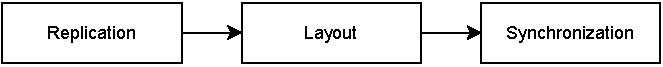
\includegraphics[keepaspectratio,width=\linewidth,height=\fullh]{diagrams/respvis-layout-process.pdf}
\caption[Layout Process of the Layouter]{
  This diagram shows the three phases of the layout process of the RespVis Layouter. 
  During the replication phase, the SVG document that shall be laid out is replicated with HTML \code{<div>} elements. 
  Afterward, these HTML elements are laid out by the browser in the layout phase, and the positions of the laid-out HTML elements are applied to their respective SVG elements during the synchronization phase.
  \imgcredit{Image created by the author of this thesis using \href{https://www.diagrams.net/}{diagrams.net}.}
}
\label{fig:LayoutProcess}
\end{figure}


During the replication process, the structure of an SVG document is replicated with HTML \code{<div>} elements. 
This replication was implemented using a hierarchical D3 data join in which the original SVG elements are bound as data objects to layout elements.
This hierarchical data join results in a counterpart in the hierarchy of layout elements for each SVG element that should be affected by the layouter.
Since not every SVG element should be positioned via the Layouter, the Layouter must know which to ignore.
For this, the \code{data-ignore-layout} and \code{data-ignore-layout-children} attributes have been introduced.
Elements that have the \code{data-ignore-layout} attribute or are children of elements that have the \code{data-ignore-layout-children} attribute will not be replicated.

To configure the layout of layout elements in CSS, it must be possible to select them uniquely with a CSS Selector.
This Selector should be as similar as possible to the Selector of the original SVG element to make it as easy as possible to configure the CSS properties of layout elements.
For this purpose, the class attributes and all data-* attributes of SVG elements are copied to their corresponding layout elements.
In addition to the classes of the replicated SVG element, the layout class is set on all layout elements.
By doing this, it is possible to specifically select the layout element of an SVG element via the same Selector by adding the layout class to the same Selector. 
If CSS rules of SVG elements use only classes and data attributes in their Selectors, the properties of corresponding layout elements can directly be configured in the same rules.
An example of how the replicated layout element tree of an SVG document looks can be seen in Listing~\ref{list:LayouterStructure}.
Furthermore, an example of CSS rules that set various properties of SVG elements and their layout elements can be seen in Listing~\ref{list:LayouterCSS}.  

\begin{samepage}
\lstinputlisting[%
  float=tp,
  aboveskip=\floatsep,
  belowskip=\floatsep,
  xleftmargin=0cm,              % no extra margins for floats
  xrightmargin=0cm,             % no extra margins for floats
  %
  basicstyle=\footnotesize\ttfamily,
  frame=shadowbox,
  numbers=left,
  label=list:LayouterStructure,
  caption={[Replicated Layout Structure of an SVG Document]%
    The replicated layout element structure of an SVG document.
    Every SVG element has a corresponding layout element that has the same classes and \code{data-*} attributes.
    In addition to the classes of the original SVG element, every layout element also has the \code{layout} class to allow specific targeting of layout elements via CSS Selectors.
  },
]{listings/layouter-structure.html}
\end{samepage}

\begin{samepage}
\lstinputlisting[%
  float=tp,
  aboveskip=\floatsep,
  belowskip=\floatsep,
  xleftmargin=0cm,              % no extra margins for floats
  xrightmargin=0cm,             % no extra margins for floats
  %
  basicstyle=\footnotesize\ttfamily,
  frame=shadowbox,
  numbers=left,
  label=list:LayouterCSS,
  caption={[CSS Rules to Style SVG]%
    These CSS rules are used to configure the layout and style of an SVG document that is being laid out by the Layouter.
    Since the Selectors of these CSS rules only use \code{class} and \code{data-*} attributes to match elements, the same rule can be used to configure the properties of an SVG element and its corresponding layout element.  
    The structure of the SVG document and its replicated layout elements can be seen in Listing~\ref{list:LayouterStructure}.
  },
]{listings/layouter-css.css}
\end{samepage}

The size of dynamically-sized elements depends on the size of their content.
Since layout elements exist separately from their SVG elements and can not access their content, a manual solution had to be implemented that sets the size of layout elements to the content size of their SVG elements when required.
An example of dynamically-sized elements is \code{<text>} elements because their size is rarely declared in absolute units and usually depends on the size of their text contents. 
The custom \code{--fit-width} and \code{--fit-height} CSS properties were introduced to activate the manual copying of dimensions from SVG elements to their layout elements. 
These boolean properties can be set in CSS rules and are being checked during the replication phase via the \code{window.getComputedStyle} method.
If at least one of these properties is set to true, the dimensions of the SVG element are calculated with the \code{Element.getBoundingClientRect} method and respectively set as \code{width} or \code{height} properties of the \code{style} attribute on the corresponding layout element.
By doing this, layout elements will have the same size as their svg elements and can be properly used in the calculation of the overall layout. 

Layout elements are automatically laid out by the browser during the layout phase of the layout process. 
Since the layout elements are simply \code{<div>} elements that have been styled in CSS rules, the browser can position them automatically via its integrated layout engine.
This positioning happens as soon as the layout elements have been rendered.
After this, the final bounding boxes of layout elements can be calculated and used for further operations.  

In the synchronization phase of the layout process, the Layouter iterates over all the layout elements, calculates their bounding boxes, and set this boundary information as attributes on the corresponding SVG elements.
Bounding boxes of layout elements are calculated relative to their parent elements using the \code{elementRelativeBounds} utility function.
This bounding box is then converted to its string representation via the \code{rectToString} utility function and set as the \code{bounds} attribute on the corresponding SVG elements. \TODO{Rename bounds attr to data-bounds}
The \code{bounds} attribute can then be deserialized to a \code{Rect} object whenever the bounding box of an SVG element is needed in subsequent renderings of SVG components. 
In addition to setting the \code{bounds} attribute of SVG elements, the Layouter also sets specific attributes on different types of SVG elements that make them fit into their calculated bounding boxes.
These attributes can, of course, be overwritten in later renderings, but they represent sensible defaults that express the boundaries of laid-out elements.
If the Layouter would not set these default attributes, they would have to be set manually on every laid-out element during the rendering process, which would be less convenient and lead to duplicated code in various places.
For SVG elements that can be mapped directly to rectangular areas, such as \code{<svg>} and \code{<rect>} elements, the Layouter sets the \code{x}, \code{y}, \code{width}, and \code{height} attributes to the values of their bounding boxes.
SVG shape elements that have explicit sizes and positions but are not rectangular, such as \code{<circle>} and \code{<line>} elements, also receive attributes that make them fit into their boundaries. 
Other SVG elements that are not explicitly sized, such as \code{<g>} and \code{<text>} elements, are merely moved to the correct position by setting their \code{transform} attribute to a translation so that their top-left corners aligns with the top-left corners of their bounding boxes. 
The Layouter does not automatically recalculate the dimensions of exactly-positioned elements based on the changed dimensions of the composite \code{<svg>} or \code{<g>} element containing them.
This has to be manually implemented in the render functions of the various components.

Using the Layouter requires a more complex rendering process than would be needed if the boundaries of elements would already be known before rendering them.
The way the Layouter works, some elements need to be rendered before calculating the layout, and afterward, when the positions and sizes of all elements are known, the visualization needs to be rendered in its final form. 
This visualization rendering process when using the Layouter consists of three phases and is shown in Figure~\ref{fig:RenderProcess}.
The three phases of the render process are the first rendering phase to render elements affecting the layout, the layouting phase, and the second rendering phase to render elements affected by the layout.
In the first rendering phase, all elements and attributes that affect the layout of a visualization need to be rendered.
This mostly includes laid-out container \code{<svg>} and \code{<g>} elements that contain exactly-positioned child elements, but it also means that the contents of dynamically-sized elements, such as \code{<text>} elements and axes, need to be fully rendered in this phase too.
The layouting phase is where all the operations of the already-described layout process are being performed.
During this phase, the bounding boxes of laid-out elements are calculated and persisted as attributes that can be accessed during the second rendering phase.
In the second rendering phase, the desired bounding box position and size of every element is known and can be used to perform a second rendering of the complete visualization.
Here, every element affected by the layout, which is every element, is rendered at its final position with its final dimensions.
In theory, the first and second rendering phases of components could be implemented in separate functions.
However, it is more convenient to invoke the same render function twice and perform some operations only if the appropriate \code{bounds} attribute has already been set.


\begin{figure}[tp]
\centering
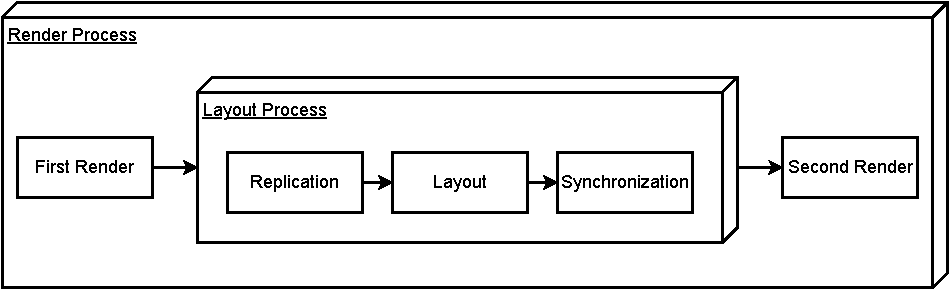
\includegraphics[keepaspectratio,width=\linewidth,height=\fullh]{diagrams/respvis-render-process.pdf}
\caption[Render Process When Using the Layouter]{
  This diagram shows the three phases of the render process when using the RespVis Layouter. 
  During the first render phase, every element that affects the layout needs to be rendered.
  The layout phase of the render process is equivalent to the layout process described in Figure~\ref{fig:LayoutProcess}.
  In this phase, the Layouter calculates the final positions and sizes of laid-out elements and stores them as attributes on the SVG elements.
  During the second render phase, all elements of the visualization are rendered at their final positions with their final dimensions by using the boundary information calculated in the layout phase.
  \imgcredit{Image created by the author of this thesis using \href{https://www.diagrams.net/}{diagrams.net}.}
}
\label{fig:RenderProcess}
\end{figure}


\subsection{Axes}

% axisData
%   scale
%   title
%     orientation
%   subtitle
%     orientation
%   configureAxis
%     d3 axis
%   default values
% axisRender
%   structure
%     .title (dynamically sized wh)
%     .subtitle (dynamically sized wh)
%     .ticks-transform (dynamically sized w or h) warum?
%       .ticks
%     laid out with CSS Grid
%   d3 axis function to render ticks
%     delete attributes and use data attributes and css to configure presentation of axis
% axisBottomRender
%   .axis-bottom
%   CSS grid with 3 rows and 1 full width column
%   title and subtitle orientations
%   tick text alignment
% axisLeftRender
%   .axis-left
%   CSS grid with 3 columns and 1 full height row
%   title and subtitle orientations
%   tick text alignment


Axes are used to visualize scales representing the mapping of abstract values to two-dimensional positions.
The implementation of all available axis components can be found in the \code{axis.ts} file in the core module.
Currently only cartesian axes are provided by the RespVis library since so far only cartesian charts have been implemented.
These cartesian axis components are distinguished by their position relative to the draw area of a visualization and at the time of writing only left and bottom axis components have been implemented in the RespVis library.
These are by far the most commonly encountered positions of cartesian axes and have been chosen because they cover most use cases. 
An axis consists of ticks, which are the actual visualization of a scale, and an optional title and subtitle, which can be rendered to additionally describe the configuration of the visualized scale. 
An example of what a rendered left and bottom axis might look like can be seen in Figure~\ref{fig:Axes}. 

\begin{figure}[tp]
\centering
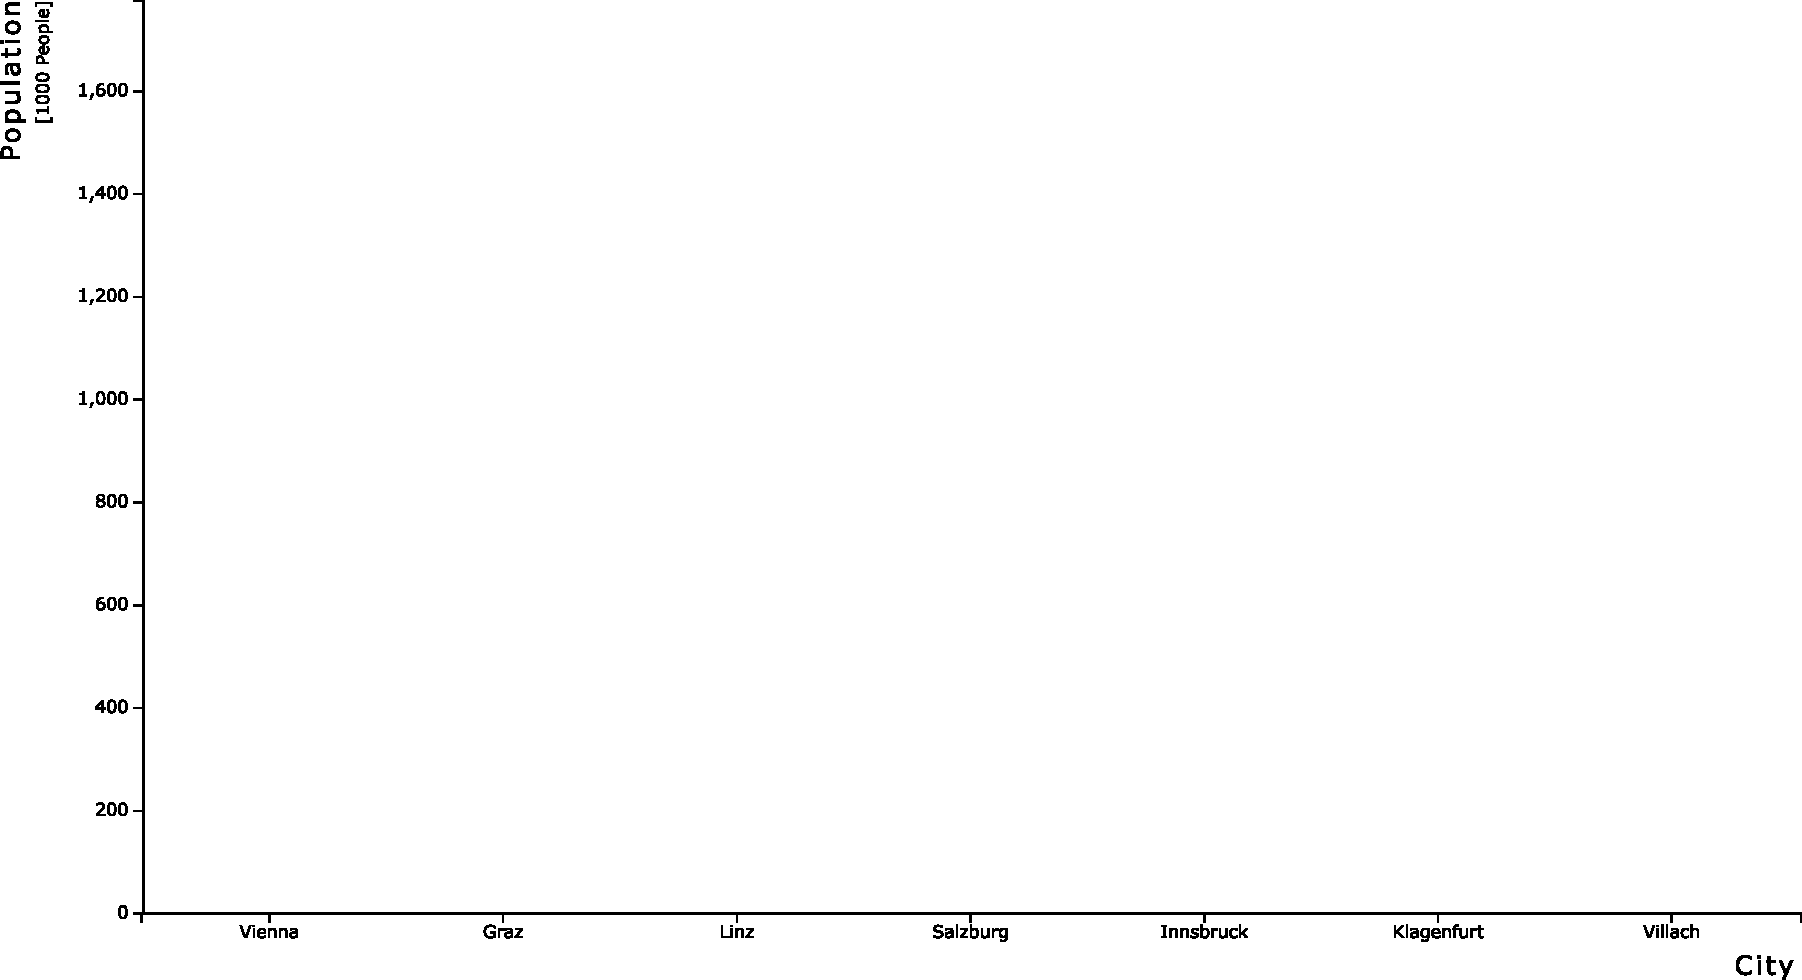
\includegraphics[keepaspectratio,width=\linewidth,height=\fullh]{diagrams/axes.pdf}
\caption[RespVis Axis Components]{
  This figure shows how a rendered left and bottom axis may look like.
  The left axis consists of a title, subtitle, and ticks, whereas the bottom axis only consists of ticks and a title. 
  \imgcredit{Image created by the author of this thesis using RespVis and \href{https://inkscape.org/}{Inkscape}.}
}
\label{fig:Axes}
\end{figure}
  

The \code{Axis} interface describes the shape of a data object with which the rendering of an axis can be configured.
It includes a \code{scale} property, which represents the scale that has to be visualized, the \code{title} and \code{subtitle} string properties, and the \code{configureAxis} function property, which can be used to configure the underlying D3 axis before rendering it.  
Like most other components, axis components consist of two main functions: a data creation function and a render function.
The \code{axisData} function is used to create a data object in the form of the \code{Axis} interface.
It is called with a \code{Partial<Axis>} object as parameter and returns a new object with all non-set but required properties of the parameter object filled with default values.
The \code{axisBottomRender} and \code{axisLeftRender} functions are used to render a left and bottom axis in a composite element on which an axis has been configured using a bound \code{Axis} data object. 
These two render functions use the non-exported \code{axisRender} base function to avoid duplicate code.
All axes have the same structure of elements which are positioned and styled as much as possible using CSS.
The root of an axis is a CSS Grid container and defines the layout of the title, subtitle and ticks elements.
The default configuration of a left axis positions these elements in a three-column layout in which the title, subtitle and ticks elements are placed in this order from left to right.
For a bottom axis, the default configuration positions the same elements in a three-row layout in which the ticks, title and subtitle elements are placed in this order from top to bottom.
Furthermore, the title and subtitle elements of a left axis are vertically oriented to save horizontal space using the \code{textOrientation} utility function.
The RespVis axis components internally use the \code{axisBottom} and \code{axisLeft} functions from the D3 axis module \parencite{D3Axis} to render the ticks of an axis.
Since these D3 functions use attributes to position and style the individual elements of the ticks of an axis, as many of these attributes as possible must be removed directly after the ticks have been rendered to allow configuration via CSS. 

\subsection{Chart}

% higher-level components that render lower-level components such as axes, legends, and series. 
% chart
%   chartRender
%     default attributes of every chart
%     .chart
%     xmlns
% chart cartesian
%   ChartCartesian
%     xAxis, Axis, data object
%     yAxis, Axis, data object
%     flipped, boolean, flipping of x and y axes
%   chartCartesianData
%     input
%       Partial<ChartCartesian> with Partial<Axis> as xAxis and yAxis type
%     default values
%   chartCartesianRender
%     chart
%     .chart-cartesian
%       .draw-area
%         .background, invisible, for capturing events
%   chartCartesianAxesRender
%      left axis with either xAxis or yAxis data depending on value of flipped
%      bottom axis with either xAxis or yAxis data depending on value of flipped
%      .x-axis
%      .y-axis
%   contents laid out with CSS grid
%     left axis, bottom axis, draw area, potential legend
%     dynamic draw-area size to fill available space

\TODO{Capitalize "Chart Component" or "Chart component"? How about only "chart" without "component"? Capitalize "Chart" everytime it's used?}
charts sind higher-level components die eine vollstaendige visualisierung inklusive achsen, legenden und series representieren.
ein beispiel eines gerenderten RespVis charts der zwei achsen, eine grouped bar series, eine label series und eine legend beinhaltet kann in Figure~\ref{fig:Chart} gesehen werden.
Ein chart wird typischerweise in dem root \code{<svg>} element eines SVG dokumentes gerendert welches zumindest die \code{chart} klasse im \code{class} attribute und den angemessenen SVG namespace im \code{xmlns} attribute gesetzt hat.
Diese attribute koennen in spezifischeren chart komponenten entweder manuel oder ueber die \code{chartRender} funktion aus der \code{chart.ts} datei im core module, welche nur diese attribute setzt, gesetzt werden.

\begin{figure}[tp]
  \centering
  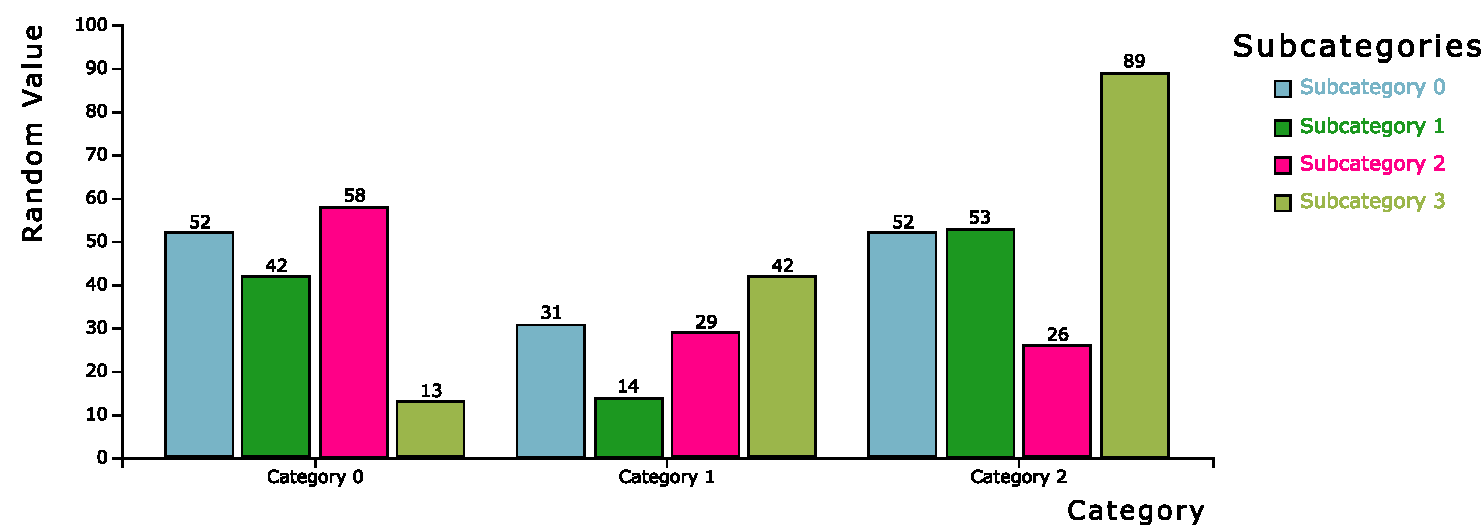
\includegraphics[keepaspectratio,width=\linewidth,height=\fullh]{diagrams/chart.pdf}
  \caption[Chart Example]{
    An example of a chart that contains two axes, a grouped bar series, a label series and a legend.
    This chart has been rendered with the RespVis library.
    \imgcredit{Image created by the author of this thesis.}
  }
  \label{fig:Chart}
\end{figure}

wie bereits erwaehnt beinhaltet die RespVis library aktuell nur die implementationen von kartesischen charts welche daten in einem kartesischen koordinatensystems visualisieren.
die implementierung der basis funktionen von kartesischen charts befindet sich in der \code{chart-cartesian.ts} datei im core module. 
das \code{ChartCartesian} interface beschreibt ein data object fuer die konfiguration von kartesischen charts.
diese data objects beinhalten die \code{xAxis} und \code{yAxis} \code{Axis} properties mit welchen jeweils die X und Y achsen des charts beschrieben werden.
das transponieren von achsen ist ein nuetzliches pattern um die responsiveness von visualisierungen zu verbessern und wird mittels des \code{flipped} boolean properties konfiguriert.
wenn das \code{flipped} property auf \code{false} gesetzt ist, wird das \code{xAxis} object fuer die konfiguration der bottom axis und das \code{yAxis} object fuer die konfiguration der left axis verwendet. 
wenn es auf \code{true} gesetzt ist, ist es genau umgekehrt.

die \code{chartCartesianData} funktion wird verwendet um ein data object in der form des \code{ChartCartesian} interface zu erzeugen.
diese funktion erhaelt ein partielles data object bei welchem nur jene properties gesetzt sind welche fuer den aufrufenden code von interesse sind.
alle nicht gesetzten properties werden mit standardwerten befuellt.
die standardwerte der \code{xAxis} und \code{yAxis} properties werden ueber die \code{axisData} funktion aus dem axis submodule gesetzt.
das \code{flipped} property wird, falls es nicht ueber den input parameter spezifiziert wird, auf \code{false} gesetzt.

das rendern von kartesischen charts ist auf zwei funktionen aufgeteilt die seperat voneinander aufgerufen werden muessen.
diese aufteilung wurde gemacht weil nicht alle teile eines kartesischen charts zum selben zeitpunkt gerendert werden koennen.
die generelle struktur eines charts muss gerendert werden bevor irgendetwas anderes gerendert werden kann da dies das draw area container element beinhaltet in welches individuelle series componenten gerendert werden muessen.
die achsen eines charts benoetigen eine vollstaendig initialisierte scale um korrekt gerendert werden zu koennen.
die range einer scale, also der wertebereich in welchen abstrakte werte gemappt werden, haengt allerdings von den dimensionen der draw area boundary ab und wird erst waehrend der render funktion der individuellen series components, welche in die draw area gerendert werden, initialisiert.    
aus diesem grund duerfen achsen erst nach allen series components gerendert werden um eine vollstaendig initialisierte scale zu gewaehrleisten.

die struktur eines kartesischen charts wird mit der \code{chartCartesianRender} funktion gerendert.
diese fuktion setzt die notwendigen chart attribute und die \code{chart} klasse mit der \code{chartRender} funktion.
Weiters wird mit dieser funktion die \code{chart-cartesian} klasse auf den root elementen der Selection gesetzt mit welcher die funktion aufgerufen wurde.
die \code{chartCartesianRender} funktion fuegt fuegt ausserdem noch ein \code{<svg>} element mit der \code{draw-area} klasse als child element des component root elementes ein.
die draw area ist das container element in welches die individuellen series components eines charts gerendert werden.
standardmaessig wird das \code{overflow} CSS property der draw area auf \code{visible} gesetzt um eventuell ueberlappende elemente nicht zu clippen.
ein \code{<svg>} element ohne tatsaechlichen content ist nicht in der lage input events abzufangen.
das bedeutet dass es zum beispiel nicht moeglich waere mittels scroll events eine zoom interaktion zu steuern wenn der cursor sich ueber der leeren flaeche der draw area befindet.
um dem entgegenzuwirken erzeugt die \code{chartCartesianRender} funktion fuer jede draw area ein transparentes \code{<rect>} background element welches die gesamte flaeche der draw area fuellt und welches es ermoeglicht input events auch in bereichen zu generieren in welchen sich keine series elemente befinden.

die \code{chartCartesianAxesRender} funktion wird verwendet um die achsen eines kartesischen charts zu rendern.
diese funktion darf nur auf elementen mit einem gebundenen \code{ChartCartesian} data object und nach der vollstaendigen initialisierung der scales, welche mit den achsen visualisiert werden sollen, aufgerufen werden.
meist bedeutet dies fuer die reihenfolge an operationen einer spezifischerer kartesischen chart component, dass zu beginn die struktur des charts mittels der \code{chartCartesianRender} funktion erzeugt werden muss, gefolgt von dem rendern der gewuenschten series components, und erst danach duerfen die achsen mittels der \code{chartCartesianAxesRender} funktion gerendert werden.
die \code{chartCartesianAxesRender} function erzeugt zwei \code{<g>} elemente und rendert eine left und eine bottom axis auf ihnen.
je nachdem ob das \code{flipped} property im gebundenen data object auf \code{true} oder \code{false} gesetzt ist, wird das \code{xAxis} data object fuer die konfiguration der bottom oder left axis verwendet und das \code{yAxis} data object jeweils fuer die andere achse.
nachdem die achsen gerendert wurden wird auf der achse auf welcher das \code{xAxis} data object gebunden ist die \code{x-axis} klasse und auf der anderen achse die \code{y-axis} klasse gesetzt. 
diese klassen werden gesetzt um die auswahl der konkreten achsen welche die jeweilige konfiguration representieren ueber CSS Selectors zu ermoeglichen.

wie es in der RespVis library ueblich ist, wird alles moegliche an positionierung und styling ueber CSS konfiguriert.
die elemente eines kartesischen charts werden ueber ein CSS Grid layout positioniert.
standardmaessig wird ein grid erzeugt welcher die \code{axis-left}, \code{axis-bottom}, \code{draw-area}, und \code{legend} areas definiert.
die groesse der meisten zeilen und spalten dieses grids ist auf \code{auto} gesetzt, was bedeutet dass deren groesse von der groesse ihres inhaltes abhaengt. 
die ausnahme hiervon sind die zeile und spalte in welchen sich die draw area befindet.
deren groesse ist auf \code{1fr} gesetzt um zu erreichen dass die draw area den gesamten restlichen horizontalen und vertikalen platz einnimmt der nicht von den anderen zeilen und spalten eingenommen wird.
die standardkonfiguration der \code{chart-cartesian} klasse sieht eine positionierung einer eventuellen legende rechts von der draw area vor.
um die position der legende zu veraendern kann entweder direkt der grid ueber CSS angepasst werden oder eine der vorkonfigurierten positionen kann ueber das \code{data-legend-position} attribut aktiviert werden.
um das setzten des \code{data-legend-position} attributes zu vereinfachen kann die \code{chartLegendPosition} funktion, welche dieses attribut auf den wert eines mitgegebenen \code{LegendPosition} enum parameters setzt, verwendet werden.


\subsection{Chart Window}

% wrappers around charts that handle the render process and add a toolbar to configure charts and perform various operations.
% chartWindowRender
%   div.chart-window
%     div.toolbar, toolbarRender
%       div.menu-tools, menuToolsRender
%         menuDropdownRender
%         no chevron
%         text unicode burger menu, trigram for heaven, https://graphemica.com/%E2%98%B0, U+2630
%     div.layouter
%   resizeEventListener
% menuDropdownRender
%   .menu
%     span.chevron, unicode, left pointing,
%     span.text
%     ul.items
%       positioning and styling via CSS
%       showing via CSS
%       highlighting via CSS

% toolFilterNominal
%   one of the tools provided by the library is the nominal filtering tool that can be used to filter a nominal dimension of the rendered data.
%   nominal data is simply labeled data where no quantitative value is assigned to the individual values.  
%   text, options, keys
%   menuDropdownRender
%   .item, seriesCheckboxRender
%     container, labels, keys
%     containerElement.checkbox
%       input[type=checkbox][id=uuid()]
%       label[for=input.id]
% tool download svg
%   dont describe in too much detail as it will be included in selected topics chapter
% resize event dispatcher

\TODO{Capitalize "Chart Window"?}
chart windows sind wrapper komponenten um charts die einen chart innerhalb eines Layouter container elementes rendern und mit einer toolbar dekorieren.
ein beispiel eines chart windows mit einem ausgeklappten tool menue in welchem sich zwei nominale filtering tools und ein svg download tool befinden kann in Figure~\ref{fig:ChartWindow} gesehen werden.
die implementierung der chart window komponente befindet sich in der \code{chart-window.ts} datei im core module.
diese komponenten stellen einen noch higher-level layer als charts dar und werden verwendet um den render prozess und die konfiguration von charts zu managen.
in den meisten anderen visualization libraries werden charts als der hoechste level an komponenten die konfiguriert werden koennen zur verfuegung gestellt.
typischerweise bedeutet das, dass zusaetzliche HTML elemente fuer die runtime configuration von charts von der einbettenden webseite selbst erzeugt und gemanaged werden muessen.     
ein chart window wird ausserhalb des SVG dokumentes eines charts auf einem HTML \code{<div>} element mit der \code{chartWindowRender} funktion gerendert.
ihre struktur besteht aus einem \code{<div>} element in welches die toolbar mit der \code{toolbarRender} funktion gerendert wird und aus einem weiteren \code{<div>} element auf welchem ein Layouter mit der \code{layouterRender} funktion initialisiert wird. 
das SVG dokument eines charts wird dann an das \code{<div>} element des Layouters als child angehaengt.

\begin{figure}[tp]
  \centering
  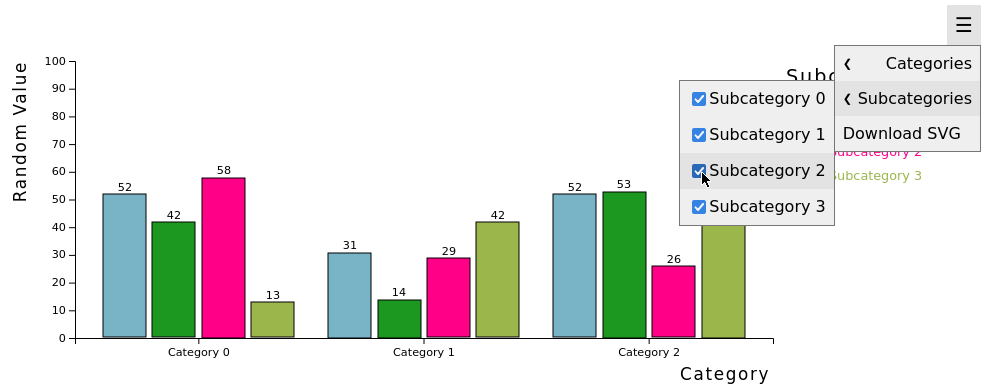
\includegraphics[keepaspectratio,width=\linewidth,height=\fullh]{images/chart-window.png}
  \caption[Chart Window Example]{
    An example of a chart that is wrapped in a chart window.
    The tool menue has been expanded by hovering over it and the menu entries of two nominal filtering tools and the download SVG tool can be seen inside.
    \imgcredit{Image created by the author of this thesis.}
  }
  \label{fig:ChartWindow}
\end{figure}


zum aktuellen zeitpunkt befindet sich in der toolbar nur das tool menu als einziges element.
das tool menu ist ein dropdown menue in welchem die einzelnen tools als menueeintraege oder als untermenues zu finden sind.
ein dropdown menu wird ueber die \code{menuDropdownRender} funktion auf den elementen der mitgegebenen Selection gerendert.
diese funktion setzt die \code{menu} klasse auf den root elementen auf welchen das dropdown menue gerendert wird.
ein dropdown menue besteht aus einem \code{<span>} element mit der \code{chevron} klasse dessen text content ein nach links zeigendes Unicode chevron symbol ist, einem zweiten \code{<span>} element mit der \code{text} klasse dessen text der titel des dropdown menues ist, und einem \code{<ul>} element mit der \code{items} klasse dass die unterelemente des dropdown menues beinhaltet.
die unterelemente eines dropdown menues werden ueber CSS absolut positioniert und angezeigt sowie highlighted solange eine hover interaktion auf dem menue stattfindet.
das tool menue wird ueber die \code{menuToolsRender} funktion erzeugt welche intern die \code{menuDropdownRender} funktion verwendet um das tool menue als dropdown menue zu initialisieren.
das root dropdown menue des tool menues wird ohne chevron symbol gerendert und enhaelt ein Unicode symbol in seinem \code{<span>} element mit der \code{text} klasse. 
das symbol dass fuer das tool menue verwendet wurde ist das \enquote{trigram for heaven} Unicode symbol mit dem code U+2630 welches haeufig fuer burger menues verwendet wird.

\TODO{Rename nominal filtering tool to categorical filtering tool}
% Categorical variables are those that have discrete categories or levels. Categorical variables can be further defined as nominal, dichotomous, or ordinal. Nominal variables describe categories that do not have a specific order to them. These include ethnicity or gender.
das core module stellt tools zur verfuegung die zu den tool menues von spezifischeren chart windows hizugefuegt werden koennen.
eines dieser tools ist das nominale filtering tool welches sich in der \code{tools/tool-filter-nominal.ts} datei im core module befindet.
dieses tool wird verwendet um eine nominale datendimension eines visualsierten datasets ueber ein dropdown menue dass eine checkbox series beinhaltet zu filtern.
nominale daten sind im gegensatz zu ordinalen daten nur gelabelte oder kategorische daten deren werten kein quantitativer wert zugewiesen ist und welche daher keine reihenfolge besitzen und auch nicht sortiert werden koennen.
das data object fuer die konfiguration eines nominalen filter tools wird durch das \code{ToolFilterNominal} interface beschrieben.
dieses interface enthaelt ein \code{text} string property welches den titel des dropdown menues definiert, ein \code{options} string array property welches die einzelnen optionen die gefiltert werden koennen definiert, und ein \code{keys} string array property welches die keys der einzelnen optionen definiert. 
die \code{toolFilterNominalData} funktion wird verwendet um ein data objekt vom typ \code{ToolFilterNominal} von einem partiellen input objekt zu erzeugen bei welchem die nicht definierten properties mit standardwerten befuellt werden.
das tool kann dann ueber die \code{toolFilterNominalRender} funktion auf einem element mit einem gebundenen \code{ToolFilterNominal} data objekt gerendert werden.
diese funktion verwendet intern die \code{menuDropdownRender} funktion um das tool als dropdown menue zu initialisieren.
die items des nominalen filter tool dropdown menues werden als eine checkbox series gerendert.

die implementierung einer checkbox series befindet sich in der \code{series-checkbox.ts} datei im core module.
eine checkbox series wird ueber ein data objekt in der form des \code{SeriesCheckbox} interfaces konfiguriert.
dieses interface beschreibt eine checkbox series ueber ein \code{container} string property mit welchem der element typ von checkbox container elementen gewaehlt werden kann, ein \code{labels} string array property mit welchem die labels der individuellen checkboxes konfiguriert werden koennen, und ein \code{keys} string array property mit welchem die keys der individuellen checkboxes definiert werden koennen.
ein data objekt von diesem typ kann mit der \code{seriesCheckboxData} funktion erzeugt werden, welche ein gueltiges objekt ausgehend von einem partiellen input objekt erstellt.
eine checkbox series wird ueber die \code{seriesCheckboxRender} funktion gerendert.
diese funktion setzt die \code{series-checkbox} klasse auf den Selection elementen, fuegt einen custom click listener hinzu welcher das toggling von checkboxes durch klicks irgendwo in ihrem container element ermoeglicht, und rendert die eigentlichen checkbox elemente durch einen D3 data join.
um den data join durchzufuehren wird ein data object pro zu rendernder checkbox benoetigt.
dies wird durch eine transformation des \code{SeriesCheckbox} data objektes in ein array von \code{Checkbox} data objekten erreicht.
jedes dieser \code{Checkbox} data objekte beinhaltet ein \code{container} property mit welchem der tag des container elementes definiert wird, ein \code{label} property und ein \code{key} property. 
alle dieser properties werden von den \code{container}, \code{labels}, und \code{keys} properties des \code{SeriesCheckbox} data objektes abgeleitet.
die \code{seriesCheckboxJoin} funktion wird mit der Selection, welche aus dem data join mit den \code{Checkbox} data objekten entsteht, aufgerufen.
diese funktion rendert die einzelnen checkboxes welche aus einem container element, einem \code{<input>} checkbox element, und aus einem \code{<label>} element bestehen.
die tags der container elemente haengen von dem werten der \code{container} properties in den gebundenen data objekten ab.
jedes container element erhaelt ausserdem die \code{checkbox} klasse und ein \code{data-key} attribut welches auf den wert des \code{key} property des data objektes gesetzt wird.
das checkbox \code{<input>} element und das \code{<label>} element werden als kinder des container elementes angehaengt.
um das \code{<label>} element dem \code{<input>} element semantisch zuzuweisen muss das \code{for} attribut am \code{<label>} element auf die id des \code{<input>} elementes gesetzt werden.
hierfuer muss jedoch zuerst jedem \code{<input>} element eine einzigartige id zugewiesen werden.
diese id wird beim erstmaligen erzeugen der checkbox ueber die die \code{uuid} funktion generiert und am \code{<input>} element als \code{id} attribut sowie auf dem \code{<label>} element als \code{for} attribut gesetzt.
die \code{uuid} funktion ist ein alias fuer die \code{v4} funktion aus dem \code{uuid} npm package \parencite{UUIDPackage}.
sie wird verwendet um UUIDs (Universally Unique IDentifiers) \parencite{UUIDRFC} der vierten version zu erzeugen welche mit enormer wahrscheinlichkeit eindeutig sind und welche daher bedenkenlos als werte fuer \code{id} attribute verwendet werden koennen.

ein weiteres tool welches vom core module zur verfuegung gestellt wird und welches von jedem chart window eingebunden wird ist das SVG download tool.
ein SVG dokument welches in ein HTML dokument einbettet ist kann nicht einfach wie ein eingebettes bild durch einen rechtsklick von benutzern heruntergeladen werden.
um ein SVG dokument zu downloaden muss dieses zuerst als string in einen \code{Blob} enkodiert werden welcher dann als object URL im \code{href} attribut auf einem \code{<a>} element gesetzt wird.
da die praesentation von RespVis visualisierungen allerdings hauptsaechlich ueber CSS konfiguriert wird, muessen die aktiven CSS properties zu attributen konvertiert werden bevor das SVG dokument gedownloaded werden kann.
um dies zu tun wird zuerst das ganze SVG dokument geklont um attribute auf den geklonten elementen setzen zu koennen ohne die gerenderte visualisierung zu beinflussen.
nachdem das dokument geklont wurde werden auf jedem geklonten element die notwendigen attribute gesetzt die den aktiven CSS properties des originalem objektes entsprechen.
die aktiven CSS properties des originalem objektes werden ueber die \code{elementComputedStyleWithoutDefaults} utility funktion berechnet.
nachdem alle notwendigen attribute auf den geklonten elementen gesetzt worden sind wird die string representation des gesamten geklonten dokumentes ueber das \code{Element.innerHTML} property berechnet und in einem \code{Blob} objekt mit dem typ \code{image/svg+xml} enkodiert.
zum aktuellen zeitpunkt wird die string representation des SVG dokumentes nicht weiter nachbearbeitet oder formatiert was zu einer recht schwer lesbaren SVG datei fuehrt und was in der zukunft verbessert werden soll. 
das \code{Blob} objekt wird dann ueber die \code{URL.createObjectURL} methode in eine URL konvertiert die ein downloadable \code{Blob} objekt representiert und im \code{href} attribut eines neu erzeugten \code{<a>} elementes gesetzt.
dieses neu erzeuge \code{<a>} element wird dann kurzzeitig an das \code{<body>} element des aktiven dokumentes angehaengt und ueber die \code{Element.click} methode geklickt was den dowload des fertig praeparierten SVG dokumentes initiiert.
die implementierung des SVG download tools befindet sich in der \code{tools/tool-download-svg.ts} datei im core module.
um dieses tool als menueeintrag des tool menues zu rendern wird die \code{toolDownloadSVGRender} funktion verwendet.
diese funktion initialisiert den menueeintrag mit der \code{tool-download-svg} klasse und einem angemessenen text content.
ausserdem setzt die \code{toolDownloadSVGRender} funktion einen click event listener auf dem menueeintrag welcher bei interaktion des benutzers den download des gerenderten SVG dokumentes ueber die \code{chartDownload} funktion initiiert.
die \code{chartDownload} funktion fuehrt dann alle bereits beschriebenen operationen aus die fuer die praeparation und den download des gerenderten SVG dokumentes notwendig sind.

\section{Legend Module}

das legend module besteht nur aus der \code{legend.ts} datei welche die implementierung einer legende beinhaltet.
eine legende wird verwendet um scales zu visualisieren deren werte nicht auf raeumliche werte in einem koordinatensystem gemappt werden.
stattdessen werden in den scales die durch eine legende visualisiert werden abstrakte werte auf visuelle eigenschaften wie zum beispiel farbe, form oder groesse abgebildet.
die legende die in diesem modul implementiert wurde visualisiert dieses mapping durch gelabelte konfigurierbare symbole.
ein beispiel welches die verwendung des legend modules demonstriert befindet sich in der \code{legend.html} datei im \code{src/examples/} ordner.
ein auszug dieses beispiels kann in Listing~\ref{list:Legend} und dessen rendering in Figure~\ref{fig:Legend} gesehen werden. 

\begin{samepage}
\lstinputlisting[%
  float=tp,
  aboveskip=\floatsep,
  belowskip=\floatsep,
  xleftmargin=0cm,              % no extra margins for floats
  xrightmargin=0cm,             % no extra margins for floats
  %
  basicstyle=\footnotesize\ttfamily,
  frame=shadowbox,
  numbers=left,
  label=list:Legend,
  caption={[Source Code of Legend Example]%
    The source code of the example website implemented in the \code{legend.html} file of the \code{src/examples/} directory that renders the three different legends seen in Figure~\ref{fig:Legend}.
    Non-essential parts of the source code have been removed to focus on the configuration of the individual legends.
    The horizontal legend has the same configuration in their data object as the rectangle symbol legend.
    The only difference between those two legends is that the items of the horizontal legend have been laid out horizontally via the \code{flex-direction: row} CSS property.
  },
]{listings/legend.html}
\end{samepage}

\begin{figure}[tp]
\centering
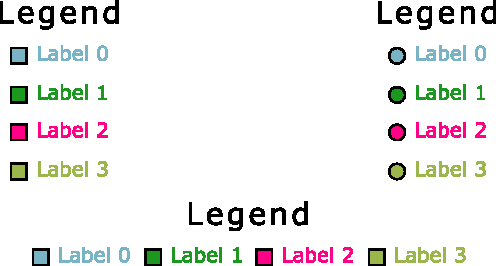
\includegraphics[keepaspectratio,width=\linewidth / 2,height=\fullh]{diagrams/legend.pdf}
\caption[Legend Example]{
  This is an example of three different legends that have been created from the source code in Listing~\ref{list:Legend}.
  One legend has been configured to have rectangles as symbols, one has been configured to have circles as symbols, and the last one has been configured with rectangle symbols but with horizontally laid out legend items.
  \imgcredit{Image created by the author of this thesis.}
}
\label{fig:Legend}
\end{figure}

ein data object mit welchem das rendering einer legende konfigurert werden kann wird durch das \code{Legend} interface beschrieben.
dieses interface beinhaltet ein \code{title} string property, ein \code{labels} string array property, ein \code{symbols} function oder function array property, ein \code{styleClasses} string oder string array property, und ein \code{keys} string array property.
der titel einer legende kann optional ueber das \code{title} property gesetzt werden.
das \code{labels} string array property definiert die labels neben den symbolen der einzelnen legend items.
die symbole der legend items werden ueber das \code{symbols} property bestimmt.
da die symbole einer legende komplett konfigurierbar sein sollen wird nicht einfach ein \code{<rect>} oder \code{<circle>} element als symbol gerendert sondern ein \code{<path>} element.
die verwendung eines \code{<path>} elementes ermoeglicht es beliebige symbole in der legende zu visualisieren.
der nachteil hiervon ist dass die konfiguration von \code{<path>} elementen aufwaendiger ist als die konfiguration von eingeschraenkteren SVG elementen.
das rendern eines symbols als \code{<path>} wird ueber eine funktion erledigt welche als input das jeweilige \code{<path>} element und die vom Layouter berechneten boundaries erhaelt.
in dem \code{symbols} property des \code{Legend} data objektes kann entweder eine einzelne solche funktion oder ein array von solchen funktionen gesetzt sein.
ist eine einzelne funktion gesetzt, erhaelt jedes symbol die selbe path konfiguration. 
sollte hier ein array an funktionen gesetzt sein, dann wird jedes symbol durch eine eigene path konfiguration visualisiert.
das \code{styleClasses} property erlaubt die konfiguration der style klassen von legend items.
eine style klasse wird in dem \code{data-style} attribut eines elementes gesetzt und dient der konfiguration von visuellen eigenschaften ueber CSS.
ein beispiel fuer verfuegbare style klassen sind die \code{categorical-0} bis \code{categorical-9} style klassen.
das setzen einer dieser klassen im \code{data-style} attribut eines elementes fuehrt dazu dass das CSS \code{fill} property auf die jeweilige kategorische farbe gesetzt wird.  
wird in dem \code{styleClasses} property eine einzelne style klasse deklariert, dann wird diese style klasse auf allen legend items gesetzt.
alternativ dazu akzeptiert dieses property auch ein array an style klassen, was dazu fuehrt das jedes legend item eine eigene style klasse gesetzt bekommt.
das \code{keys} property eines \code{Legend} data objektes bestimmt die werte der \code{data-key} attribute der einzelnen legend items.
ein data objekt das der form des \code{Legend} interface entspricht kann mit der \code{legendData} funktion erzeugt werden.
diese funktion erhaelt ein input objekt von dem selben typ wie jener den sie erzeugt bei welchem die werte die fuer den aufrufenden code nicht von interesse sind nicht gesetzt sein muessen und mit standardwerten befuellt werden.

eine legende wird mit der \code{legendRender} funktion auf elementen gerendert auf denen ein \code{Legend} data objekt gebunden ist.
diese funktion setzt die \code{legend} klasse auf den elementen der uebergebenen Selection.
innerhalb des root elementes der legende befindet sich ein \code{<text>} element mit der \code{text} klasse welches den titel der legende representiert, und ein \code{<g>} element mit der \code{items} klasse in welches die einzelnen legend items ueber einen data join gerendert werden.
um den legend item data join durchzufuehren benoetigt man ein data objekt pro legend item das gerendert werden soll.
dieses array an \code{LegendItem} data objekten, welche aus den \code{label}, \code{styleClass}, \code{symbol}, und \code{key} eigenschaften bestehen, wird durch transformation des \code{Legend} data objektes erzeugt.
ueber einen data join mit diesem array an data objekten wird fuer jedes legend item ein \code{<g>} element mit der \code{legend-item} klasse erzeugt.
an jedes dieser \code{<g>} elemente werden dann ein \code{<path>} element mit der \code{symbol} klasse und ein \code{<text>} element mit der \code{label} klassen angehaengt.
das \code{label} property des gebundenen \code{LegendItem} data objektes wird dann als textinhalt des \code{<text>} elementes gesetzt und das \code{symbol} property wird verwendet um die form des \code{<path>} objektes zu bestimmen.
ausserdem werden die \code{data-style} und \code{data-key} attribute auf dem \code{<g>} legend item element auf die werte der \code{styleClass} und \code{key} eigenschaften des data objektes gesetzt.
im kern kann eine legende auch als legend item series angesehen werden und wie auch alle anderen series components kann auch in den data join der legende direkt ueber die \code{enter}, \code{update}, und \code{exit} events, welche auf dem root element der legende gesendet werden, eingegriffen werden.
die event objekte dieser events beinhalten im \code{detail.selection} property jeweils die enter, update, und exit Selections des darunterliegenden data joins.
ueber diese properties koennen beliebige operationen in den verschiedenen phasen des data joins ausgefuehrt werden.


\TODO{Capitalize "Core Module", "Bar Module", "Chart", "Chart Component", "Axis", "Axis Component" according to Keith}




\section{Tooltip Module}
\label{sec:TooltipModule}

\TODO{Capitalize "Tooltip", "Tooltip Module", ...}

tooltips werden verwendet um zusaetzliche informationen eines elementes anzuzeigen die zu umfangreich sind um sie permanent anzuzeigen.
eine visualisierung die zu viele informationen zur selben zeit darstellt verliert an effektivitaet da ein groesserer kognitiver aufwand aufgebracht werden muss um sie zu interpretieren.
durch die verwendung von tooltips kann dieses problem dadurch geloest werden dass zu detailierte informationen erst durch interaktion der benutzter mit einem element in dessen kontext die information steht angezeigt werden.
ausserdem ist es fuer tooltips ok andere wichtige teile einer visualisierung zu ueberdecken da sie nicht permanent sichbar sind.
ein beispiel eines bar charts in welchem zusaetzliche informationen ueber einen tooltip angezeigt werden kann in Figure~\ref{fig:Tooltip} gesehen werden.

\begin{figure}[tp]
\centering
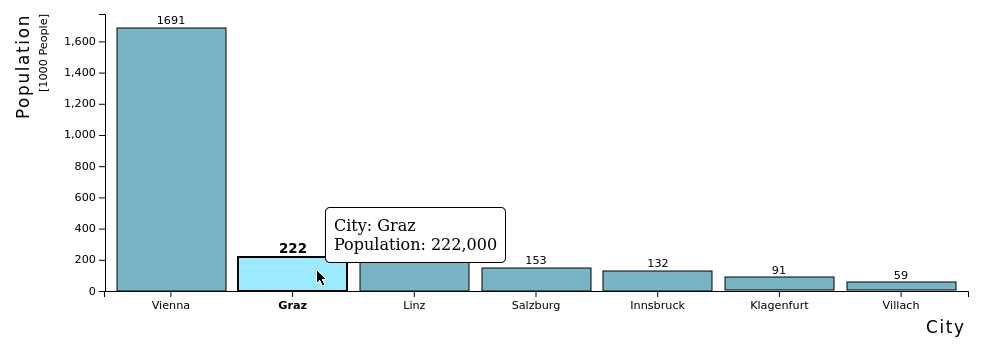
\includegraphics[keepaspectratio,width=\linewidth,height=\fullh]{images/tooltip.png}
\caption[Tooltip Example]{
  A bar chart with a tooltip showing additional information of the data record associated with an individual bar.
  Since the tooltip is only visible while the user interacts with the context element, it is ok that the tooltip covers other important parts of the visualization.
  \imgcredit{Image created by the author of this thesis.}
  }
  \label{fig:Tooltip}
\end{figure}
  
  
das tooltip module befindet sich im \code{src/lib/tooltip/} odner des projektes.
die hauptdatei welche die implementierung der tooltip funktionalitaet beinhaltet ist die \code{tooltip.ts} datei.
so wie tooltips hier implementiert wurden, wird die gleichzeitige anzeige mehrerer tooltips unterstuetzt.
um dies zu erreichen, erwarten alle funktionen die tooltip operationen ausfuehren, dass das tooltip element auf welchem die operation ausgefuehrt werden soll als erster parameter an die funktion uebergeben wird.
diese funktionen erlauben es allerdings auch ein \code{null} objekt in diesem parameter zu uebergeben, was zur verwendung eines standard tooltip elementes, welches an das \code{<body>} element des aktiven dokumentes angehaengt wird, fuehrt.
%
tooltips sind HTML \code{<div>} elemente mit der \code{tooltip} klasse und werden ueber CSS gestyled.
der inhalt eines tooltips wird mit der \code{tooltipContent} funktion gesetzt.
diese funktion erlaubt es den inhalt eines tooltips als string zu definieren welcher als HTML inhalt des tooltip elementes gesetzt wird.
%
die position eines tooltips wird ueber die \code{tooltipPosition} funktion gesetzt.
diese funktion erhaelt ein objekt als parameter mit welchem die position in viewport koordinaten und ein optionaler offset von dieser position bestimmt werden.
wird kein expliziter offset gefordert berechnet die \code{tooltipPosition} funktion einen welcher den tooltip so postioniert dass er immer in dem sichtbaren bereich des browsers positioniert wird.
tooltips werden ueber viewport koordinaten positioniert und die endgueltige position eines tooltips wird ueber die CSS \code{top}, \code{bottom}, \code{left}, und \code{right} eigenschaften gesetzt.
welche dieser eigenschaften verwendet wird haengt von der offset richtung des tooltips ab. 
%
tooltips werden mit der \code{tooltipShow} funktion angezeigt und mit der \code{tooltipHide} funktion versteckt.
diese funktionen setzen und enfernen jeweils die \code{show} klasse von dem tooltip element wodurch die CSS \code{opacity} eigenschaft des elementes beinflusst wird. 

neben der \code{tooltip.ts} datei beinhaltet das tooltip modul noch die \code{series-config-tooltips.ts} datei.
in dieser datei befindet sich keine eigene komponente sondern utility funktionen um die konfiguration und das handling von tooltips auf series komponenten zu vereinfachen.
die datenobjekt interfaces von series komponenten mit welchen tooltips konfiguriert werden sollen koennen von dem \code{SeriesConfigTooltips} interface erben.
dieses interface beinhaltet die \code{tooltipsEnabled}, \code{tooltips}, und \code{tooltipPositions} eigenschaften.
die \code{tooltipsEnabled} boolean eigenschaft ermoeglicht das aktivieren und deaktivieren von tooltips.
der inhalt der tooltips von individuellen series item elements wird ueber die \code{tooltips} eigenschaft konfiguriert.
in dieser eigenschaft wird eine funktion gesetzt die mit dem series item element aufgerufen wird fuer welches ein tooltip angezeigt werden soll und welche den tooltipinhalt als string zurueckliefert.     
die positionen der einzelnen tooltips werden ueber die \code{tooltipPositions} eigenschaft gesetzt.
der wert dieser eigenschaft ist ebenfalls eine funktion welche mit dem kontext series item element und der aktuellen mausposition in viewport koordinaten als parameter aufgerufen wird.
die gewuenschte position des tooltips kann dann ueber diese parameter berechnet werden.
%
zusaetzlich zu dem \code{SeriesConfigTooltips} interface kann die \code{seriesConfigTooltipsHandleEvents} funktion in der \code{series-config-tooltips.ts} datei gefunden werden.
diese funktion kann in series komponenten verwendet werden um \code{mouseover}, \code{mousemove}, und \code{mouseout} event listener an die root elemente einer series anzuhaengen die fuer das management von tooltips zustaendig sind.
diese event listener verwenden die \code{SeriesConfigTooltips} eigenschaften der an den series elementen gebundenen datenobjekte um die sichtbarkeit, den inhalt, und die position von tooltips zu modifizieren.
die verwendung dieser utility typen und funktionen ist optional.
es steht series komponenten frei eigene eigenschaften fuer die konfiguration von tooltips zur verfuegung zu stellen und das handling von tooltips selbst zu implementieren.
allerdings ist es aus konsistenzgruenden besser wenn sich die art der konfiguration von tooltips nicht zu sehr zwischen unterschiedlichen series komponenten unterscheidet.   



\section{Bar Module}

das bar modul befindet sich in dem \code{src/lib/bars/} ordner des projektes und beinhaltet komponenten um unterschiedliche arten von bar charts zu rendern.
bar charts werden zur visualisierung von kategorischen datensaetzen durch rectangles eingesetzt wobei die laenge der rectangles proportional zu den werten einer quantitativen datendimension ist.
in einem kategorischen datensatz ist eine kategorie eindeutig anderen dimensionen der einzelnen dateneintraege zuordenbar.
ein beispiel hierfuer waere ein datensatz in welchem unterschiedliche charakteristiken einzelner laender aufgelistet sind.
bar charts gehoeren zu den aeltesten arten von charts mit einem der ersten aufkommen in \textcite{CommercialAndPoliticalAtlas} und gehoeren auch heute noch zu den am haeufigsten vorgefundenen visualisierungen (\~36\% der 378 studied charts by \textcite{DesignPatternsTradeOffsRespVisGallery}) im modernen web.
die bars einens bar charts koennen entweder horizontal oder vertikal ausgerichtet sein.
bei einem horizontalen bar chart, manchal auch row chart genannt, wird die quantitative dimension ueber die X achse ausgedrueckt.
diese variante von bar charts eignet sich besser fuer die darstellung in layouts mit eingeschraenkter breite, da die labels der kategorischen achse leichter ohne zu ueberlappen positioniert werden koennen und da ein horizontaler bar chart vertikal gescrollt werden kann was horizontalem scrollen zu bevorzugen ist.
im gegensatz zu horizontalen bar charts wird bei vertikalen bar charts, manchmal auch column charts genannt, die quantitative dimension ueber die Y achse ausgedrueckt. 
das bar modul beinhaltet komponenten fuer das rendering von basic, grouped, und stacked bar charts welche in unterschiedlichen visualisierungsszenarien eingesetzt werden koennen.
fuer jede art von bar chart wird eine Series Component, eine Chart Component und eine Chart Window Component zur verfuegung gestellt. 
die implementierung der unterschiedlichen arten von bar charts und wann welche art am besten zur anwendung kommt wird in den folgenden sections beschrieben.

\subsection{Basic Bars}

\TODO{Is "Basic Bars" a good name? Maybe "Single Bars" or "Bars" or something else?}

\TODO{Add figure of vertical and horizontal bar charts (subfigures?)}

basic bar charts, manchmal auch single-series bar charts genannt, werden verwendet um unterschiede einer quantitativen dimension verschiedener kategorien eines kategorischen datensatzes zu verdeutlichen.
von jedem dateneintrag wird jeweils eine kategorische und eine quantitative dimension als eine bar visualisiert, wobei die zu visualisierenden kategorien eindeutig auf einen quantitativen wert gemapped werden koennen muessen.
die kategorien eines bar charts werden ueber eine band scale auf raeumliche dimensionen gemapped.
eine band scale wird verwendet um werte gleichmaessig auf gleich grosse intervalle (baender) des verfuegbaren platzes aufzuteilen. 
der abstand zwischen den einzelnen intervallen ist konfigurierbar.
die breite der zu rendernden bars ergibt sich durch die anzahl der kategorien, dem bereich auf welchen sie ueber die band scale aufgeteilt werden sollen, und dem abstand zwischen den bars. 
die quantitativen werte, welche die laenge der individuellen bars bestimmen, werden ueber eine continuous scale auf raemliche dimensionen gemapped.
eine continuous scale bildet abstrakte quantitative werte ueber eine kontinuierliche interpolationsfunktion auf den bereich zwischen zwei extemen ab.
in den meisten faellen kommt eine lineare interpolation ueber eine linear scale zur anwendung.
es steht dem author einer visualisierung jedoch frei eine andere form der interpolation, wie zum beispiel eine logarithmische funktion ueber eine logarithmic scale, zu waehlen. 

die lowest-level komponente die fuer das rendern eines bar charts notwendig ist ist eine bar series.
eine bar series ist eine sammlung von \code{<rect>} elementen welche die bars innerhalb der draw area eines bar charts representieren.
die implementierung der bar series komponente befindet sich in der \code{series-bar.ts} datei des bar moduls.
das datenobjekt fuer die konfiguration einer bar series wird ueber das \code{SeriesBar} interface beschrieben.
diese interface beschreibt ein objekt mit den \code{categories}, \code{values}, \code{categoryScale}, \code{valueScale}, \code{flipped}, \code{styleClasses}, und \code{keys} eigenschaften.
zusaetzlich zu diesen eigenschaften wird die konfiguration von tooltips ueber die eigenschaften des \code{SeriesConfigTooltips} interface, welches in Section~\ref{sec:TooltipModule} beschrieben wird, ermoeglicht.
die \code{categories} und \code{values} eigenschaften sind arrays welche die individuellen kategorien und deren quantitative werte repraesentieren.
das mapping der kategorischen und quantitativen werte auf raeumliche dimensionen wird ueber die \code{categoryScale} und \code{valueScale} eigenschaften bestimmt.
ob vertikale oder horizontale bars gerendert werden haengt von dem wert der \code{flipped} eigenschaft ab, wobei ein wert von \code{false} fuer vertikale bars und ein wert von \code{true} fuer horizontale bars steht.
die \code{data-style} attribute, welche die farbe von bars bestimmen, und die \code{data-key} attribute, welche zur identifikation von zusammengehoerenden elementen verwendet werden, werden ueber die \code{styleClasses} und \code{keys} eigenschaften bestimmt.
ein mit standardwerten initialisiertes \code{SeriesBar} datenobjekt kann mit der \code{seriesBarData} funktion von einem partiellen input objekt erzeugt werden.
diese datenobjekte koennen an \code{<svg>} oder \code{<g>} elemente gebunden werden in welche dann eine bar series mit der \code{seriesBarRender} funktion gerendert werden kann.
die individuellen bar elemente werden ueber einen data join mit einem array an \code{Bar} datenobjekten erzeugt, welches durch transformation des gebundenen \code{SeriesBar} datenobjektes berechnet wird.
die position und groesse der bars wird mithilfe der beiden scales berechnet deren output values auf die dimensionen der bounding box des series elementes gemapped werden, welche vom Layouter berechnet und im \code{bounds} attribut gespeichert wurden.
jede bar hat eine enter und exit transition und ihre position und groesse wird ueber eine update transition zwischen aktuellen und neuen werten interpoliert.
diese transitions erleichtern es aenderungen in den visualisierten daten nachzuvollziehen und fuehren zu einer verbesserung der user experience.
wie bei alle anderen series komponenten, werden die enter, update, und exit events mit der jeweiligen Selection des bar data joins auf dem root element der series dispatched um das injezieren von eigenem verhalten in die verschiedenen phasen des data joins zu ermoeglichen. 

die implementierung von bar charts befindet sich in der \code{chart-bar.ts} datei im bar modul. 
bar charts sind kartesische charts die eine bar series mit optionalen labels in ihrer draw area rendern.
das \code{ChartBar} interface beschreibt die form von datenobjekten fuer die konfiguration von bar charts.
es beinhaltet alle eigenschaften der \code{ChartCartesian} und \code{SeriesBar} interfaces und fuegt zusaetzliche eigenschaften zur konfiguration von bar labels hinzu. 
ein mit standardwerten initialisiertes datenobjekt vom typ \code{ChartBar} kann mit der \code{chartBarData} funktion von einem partiellen input objekt erzeugt werden.
nachdem solch ein datenobjekt auf einem \code{<svg>} oder \code{<g>} element gebunden wurde, kann ein bar chart mit der \code{chartBarRender} funktion in dieses element gerendert werden.
diese funktion initialisiert einen kartesischen chart, initialisiert und rendert eine bar series und eine optionale label series in der draw area des charts, und rendert die scales mit welchen die bar series gerendert wurde als left und bottom axes des charts. 
weiters werden \code{mouseover} event listener an die bar series angehaengt die fuer das hervorheben von bars und den dazugehoerigen ticks auf der category axis zustaendig sind.

ein bar chart window ist die highest-level komponente die verwendet werden kann um einen bar chart zu rendern der in ein Layouter element eingebettet wird um dessen elemente ueber CSS zu positionieren.
ueber die toolbar des bar chart windows koennen die kategorien des bar charts gefiltert und das SVG dokument des bar charts gedownloaded werden.
das datenobjekt fuer die konfiguration eines bar chart windows wird durch das \code{ChartWindowBar} interface beschrieben.
dieses interface erbt vom \code{ChartBar} interface und beinhaltet dadurch alle eigenschaften die fuer die konfiguration des darunterliegenden bar charts benoetigt werden.
zusaetzlich zu diesen, werden weitere eigenschaften fuer das filtern von kategorien, wie etwa die derzeit aktiven kategorien und das verhalten der value scale, zur verfuegung gestellt.
die \code{chartWindowBarData} funktion kann verwendet werden um ein datenobjekt fuer die konfiguration eines bar chart windows von einem partiellen input objekt zu erzeugen bei welchem die nicht definierten werte mit standardwerten initialisiert werden.
mit der \code{chartWindowBarRender} funktion kann ein bar chart window in einem \code{<div>} element auf welchem ein angemessenes datenobjekt gebunden is gerendert werden.
diese funktion rendert die toolbar mit den kategorie filter und SVG download tools, initialisiert den eingebetteten chart mit den gefilterten werten des chart window datenobjektes, und rendert den chart, entsprechend des render prozesses definiert in Section~\ref{sec:Layouter}, zweimal mit einem layout computation schritt dazwischen.
standardmaessig wird das chart window nicht automatisch rerendert wenn sich die groesse des viewports aendert oder wenn die aktiven kategorien gefiltert werden.
das rerendern bei viewport groessenaenderungen kann ueber einen \code{resize} event listener auf dem chart window root element implementiert werden in welchem die chart window render funktion erneut aufgerufen wird nachdem das gebundene datenobjekt angemessen an die neuen dimensionen des viewports angepasst wurde.
das bar chart window sendet ein \code{categoryfilter} event mit den derzeit aktiven kategorien immer wenn kategorien ueber das filter tool aktiviert oder deaktiviert werden.
um den bar chart auf die neue filterkonfiguration anzupassen muss ein \code{categoryfilter} event listener implementiert werden welcher die aktiven kategorien im datenobjekt des chart windows aktualisiert und das chart window rerendert.
muessen keine speziellen konfigurationen bei aenderung der viewport groesse oder des kategoriefilters durchgefuehrt werden, koennen die \code{chartWindowBarAutoResize} und \code{chartWindowBarAutoFilterCategories} funktionen verwendet werden um \code{resize} und \code{categoryfilter} event listener an das chart window anzuhaengen die das standardverhalten implementieren.
ein simples beispiel dafuer wie ein skalierendes bar chart window erzeugt werden kann welches das filtern von kategorien erlaubt ist in Listing~\ref{list:BarChartWindow} ersichtlich.
die resultierende visualisierung dieses codes kann in Figure~\ref{fig:BarChartWindow} gesehen werden.

\begin{samepage}
\lstinputlisting[%
  float=tp,
  aboveskip=\floatsep,
  belowskip=\floatsep,
  xleftmargin=0cm,              % no extra margins for floats
  xrightmargin=0cm,             % no extra margins for floats
  %
  basicstyle=\footnotesize\ttfamily,
  frame=shadowbox,
  numbers=left,
  label=list:BarChartWindow,
  caption={[Bar Chart Window Example]%
    The example source code that creates a Bar Chart Window.
    The Bar Chart Window is configured with the bound data object that is initialized via the \code{chartWindowBarData} function.
    After configuration, the Chart Window is rendered by the \code{chartWindowBarRender} function.
    Since no special responsive behavior is desired in this example, the default resize and category filter behavior is attached to the Chart Window via the \code{chartWindowBarAutoResize} and \code{chartWindowBarAutoFilterCategories} functions. 
  },
]{listings/bar-chart-window.js}
\end{samepage}
  

\begin{figure}[tp]
\centering
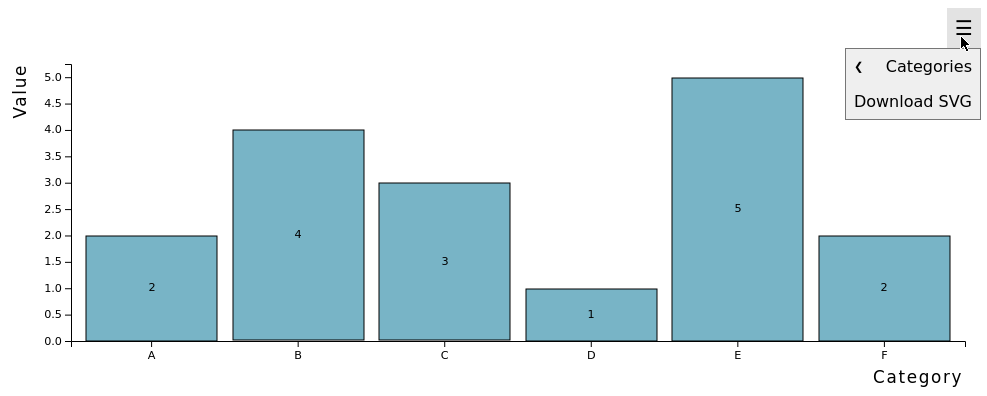
\includegraphics[keepaspectratio,width=\linewidth,height=\fullh]{images/bar-chart-window.png}
\caption[Bar Chart Window Example]{
  The resulting Bar Chart of the example code in Listing~\ref{list:BarChartWindow}. 
  \imgcredit{Image created by the author of this thesis using RespVis.}
}
\label{fig:BarChartWindow}
\end{figure}



\subsection{Grouped Bars}

ein grouped bar chart, manchmal auch clustered oder multi-series bar chart genannt, wird verwendet um mehrere quantitative dimensionen unterschiedlicher kategorien eines kategorischen datensatzes miteinander zu vergleichen.
in einem solchen chart wird fuer jede kategorie eine gruppe an bars gerendert deren laengen proportional zu den werten der unterschiedlichen quantitativen dimensionen sind.
die verschiedenen zu visualisierenden quantitativen dimensionen muessen miteinander vergleichbar sein und koennen als unterkategorien der einzelnen kategorien betrachtet werden.
wie bei basic bar charts werden auch hier die kategorien ueber band scales auf raeumliche dimensionen abgebildet.
der unterschied befindet sich darin dass bei grouped bar charts zwei verschiedene band scales zur anwendung kommen.
ueber die category scale wird der verfuegbare platz der draw area auf die anzahl der kategorien aufgeteilt und ueber die subcategory scale wird der platz innerhalb der daraus resultierenden gleich grossen intervalle auf die anzahl der unterkategorien aufgeteilt.
das abbilden von quantitativen werten auf raeumliche dimensionen wird wieder ueber eine continuous scale durchgefuehrt, wobei die selbe scale fuer jeden wert verwendet werden muss damit die werte miteinander vergleichbar sind.

fuer das rendering von grouped bar charts werden drei verschiedene komponenten zur verfuegung gestellt welche ihren gegenstuecken fuer das rendering von basic bar charts sehr aehnlich sind.
die grouped bar series ist die lowest-level komponente die dafuer gedacht ist eine sammlung an \code{<rect>} elementen, welche die jeweiligen werte und kategorien eines grouped bar charts representieren, in die draw area eines charts zu rendern.
der unterschied einer grouped bar series zu einer basic bar series ist dass zusaetzliche eigenschaften fuer die konfiguration der unterkategorien notwendig sind und dass manche bereits vorhandene eigenschaften hier zwei-dimensionale arrays erfordern um deren werte den hier zwei-dimensional (kategorie/unterkategorie) gruppierten bars zuzuordnen.
allen bars die der selben unterkategorie angehoeren werden die selben style klassen zugewiesen um die werte der einzelnen kategorien leichter miteinander vergleichen zu koennen.
ein grouped bar chart ist ein kartesischer chart mit einer grouped bar series und optionalen labels in seiner draw area, einer left und bottom axis die die scales der grouped bar series visualisieren, und einer legende die die unterkategorien des charts beschreibt.
ein solcher Chart implementiert ausserdem event listener auf unterschiedlichen elementen die das gemeinsame hervorheben von zusammengehoerenden bars, labels, category axis ticks, und legend items abwickeln.  
ein Grouped Bar Chart Window ist die highest-order komponente die verwendet werden kann um einen Grouped Bar Chart zu rendern.
diese komponente plaziert den Chart innerhalb eines Layouters und managed den render prozess der es erlaubt individuelle elemente ueber CSS zu positionieren.
weiters dekoriert ein solches Chart Window den Grouped Bar Chart mit einer toolbar in welcher sich ein SVG download tool und zwei filter tools befinden um die visualisierten kategorien und unterkategorien zu filtern.
die konfiguration des eingebetteten Charts mit den gefilterten eigenschaften des am Chart Window gebundenen datenobjektes wird von der render funktion des Grouped Chart Windows durchgefuehrt.
immer wenn der user mit den filter tools interagiert und die zusammenstellung der aktiven kategorien und unterkategorien veraendert werden die \code{categoryfilter} und \code{subcategoryfilter} events mit jeweils den neuen aktiven kategorien und unterkategorien ausgesandt.
der author der visualisierung kann entweder spezielles verhalten in eigenen resize und filter event listenern implementieren oder das standardverhalten ueber die zur verfuegung gestellten \code{chartWindowBarGroupedAutoResize}, \code{chartWindowBarGroupedAutoFilterCategories}, und \code{chartWindowBarGroupedAutoSubcategories} funktionen aktivieren.
der beispielcode um einen einfachen grouped bar chart zu erzeugen welcher sich an die groesse seines container elementes anpasst und in welchem die kategorien und unterkategorien ueber die toolbar gefiltert werden koennen befindet sich in Listing~\ref{list:GroupedBarChartWindow}.
die resultierende visualisierung dieses beispiels kann in Figure~\ref{fig:GroupedBarChartWindow} gesehen werden.  

\begin{samepage}
\lstinputlisting[%
  float=tp,
  aboveskip=\floatsep,
  belowskip=\floatsep,
  xleftmargin=0cm,              % no extra margins for floats
  xrightmargin=0cm,             % no extra margins for floats
  %
  basicstyle=\footnotesize\ttfamily,
  frame=shadowbox,
  numbers=left,
  label=list:GroupedBarChartWindow,
  caption={[Grouped Bar Chart Window Example]%
    The example source code that creates a Grouped Bar Chart Window.
    The Grouped Bar Chart Window is configured with the bound data object that is initialized via the \code{chartWindowBarGroupedData} function.
    After configuration, the Chart Window is rendered by the \code{chartWindowBarGroupedRender} function.
    Since no special responsive behavior is desired in this example, the default resize, category filter, and subcategory filter behavior is attached to the Chart Window via the \code{chartWindowBarGroupedAutoResize}, \code{chartWindowBarGroupedAutoFilterCategories}, and \code{chartWindowBarGroupedAutoFilterSubcategories} functions. 
  },
]{listings/grouped-bar-chart-window.js}
\end{samepage}
    
  
\begin{figure}[tp]
\centering
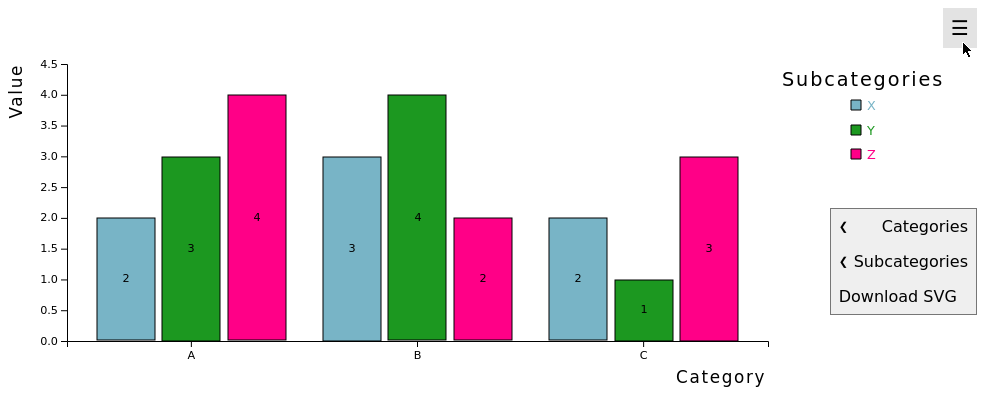
\includegraphics[keepaspectratio,width=\linewidth,height=\fullh]{images/grouped-bar-chart-window.png}
\caption[Grouped Bar Chart Window Example]{
  The resulting Grouped Bar Chart of the example code in Listing~\ref{list:GroupedBarChartWindow}. 
  The tool menu popup has manually been displaced to not cover the legend. 
  \imgcredit{Image created by the author of this thesis using RespVis.}
}
\label{fig:GroupedBarChartWindow}
\end{figure}

\subsection{Stacked Bars}

ein stacked bar chart wird verwendet um die relativen beitraege mehrerer quantitativer dimensionen zu einem kombinierten gesamten von unterschiedlichen kategorien eines kategorischen datensatzes miteinander zu vergleichen.
die quantitativen dimensionen koennen als unterkategorien der einzelnen kategorien gesehen werden und muessen in einer part-to-whole beziehung zueinander stehen.
Stacked Bar Charts existieren in zwei verschiedenen variationen: Basic Stacked Bar Charts und Percent Stacked Bar Charts.
bei Basic Stacked Bar Charts werden alle bars einer kategorie einfach uebereinander platziert was bedeutet dass die kombinierten gesamten unterschiedlicher kategorien miteinander verglichen werden koennen.
die laengen eines Percent Stacked Bar Charts werden hingegen nur als prozentuelle anteile eines gesamten betrachtet.
das kombinierte gesamte jeder kategorie eines solchen Charts betraegt immer genau 100\% wodurch zwar die information ueber die summe aller werte einer kategorie verloren geht aber die beitraege der einzelnen werte zu dem gesamten klarer ersichtlich ist.
alle bars innerhalb einer kategorie werden uebereinander platziert und die bars die der selben unterkategorie angehoeren haben den selben style.
das abbilden von kategorien und quantitativen werten auf raeumliche dimensionen wird so wie bei Basic Bar Charts ueber eine band scale und eine continuous scale erreicht.
der unterschied besteht darin, dass der ursprung von bars nicht auf dem unteren extrem der value scale liegt sondern sich aus der summe der laengen der vorhergegangenen bars derselben kategorie ergibt.

die RespVis library stellt drei verschiedene komponenten unterschiedlicher layer fuer das rendern von Stacked Bar Charts zur verfuegung.
die Stacked Bar Series, Stacked Bar Chart und Stacked Bar Chart Window komponenten sind ihren gegenstuecken fuer das rendern von Grouped Bar Charts sehr aehnlich.
auch bei diesen komponenten werden bars ueber die zwei-dimensionale (kategorie/unterkategorie) gruppierung von quantitativen werten gerendert, wobei eigenschaften welche individuelle bars beeinflussen ebenfalls als ein zwei-dimensionales array konfiguriert werden koennen.
der hauptunterschied in der implementierung der Stacked Bar Series von der Grouped Bar Series besteht in der berechnung der positionen und ausmasse von bars.
Stacked Bar Charts sind, so wie Grouped Bar Charts, kartesische Charts die aus einer Stacked Bar Series mit optionalen labels, zwei achsen, und einer legende bestehen.
Stacked Bar Chart Windows sind ebenfallst äquivalent zu ihren Gegenstuecken von Grouped Bar Charts und rendern einen Stacked Bar Chart innerhalb eines Layouters unter einhaltung des erforderlichen render prozesses waehrend in der toolbar tools fuer das filtern der kategorien und unterkategorien des gerenderten Charts zur verfuegung gestellt werden.
um das rendern eines Percent Stacked Bar Charts zu vereinfachen, koennen die quantitativen werte in dem datenobjekt eines Stacked Bar Chart Windows ueber die \code{valuesAsRatios} boolean eigenschaft als anteile deklariert werden was dazu fuehrt dass werte in prozentuelle anteile ihrer summen innerhalb einer kategorie transformiert werden.
in Listing~\ref{list:StackedBarChartWindow} ist der notwendige code ersichtlich mit dem ein skalierendes Stacked Bar Chart Window erzeugt werden kann dessen kategorien und unterkategorien ueber die toolbar gefiltert werden koennen.
das gerenderte resultat dieses codes kann in Figure~\ref{fig:StackedBarChartWindow} gesehen werden.


\begin{samepage}
\lstinputlisting[%
  float=tp,
  aboveskip=\floatsep,
  belowskip=\floatsep,
  xleftmargin=0cm,              % no extra margins for floats
  xrightmargin=0cm,             % no extra margins for floats
  %
  basicstyle=\footnotesize\ttfamily,
  frame=shadowbox,
  numbers=left,
  label=list:StackedBarChartWindow,
  caption={[Stacked Bar Chart Window Example]%
    The example source code that creates a Stacked Bar Chart Window.
    The Stacked Bar Chart Window is configured with the bound data object that is initialized via the \code{chartWindowBarStackedData} function.
    After configuration, the Chart Window is rendered by the \code{chartWindowBarStackedRender} function.
    Since no special responsive behavior is desired in this example, the default resize, category filter, and subcategory filter behavior is attached to the Chart Window via the \code{chartWindowBarStackedAutoResize}, \code{chartWindowBarStackedAutoFilterCategories}, and \code{chartWindowBarStackedAutoFilterSubcategories} functions. 
  },
]{listings/stacked-bar-chart-window.js}
\end{samepage}
  
\begin{figure}[tp]
\centering
\subfloat[Basic Stacked Bar Chart]{%
\hspace{1cm}
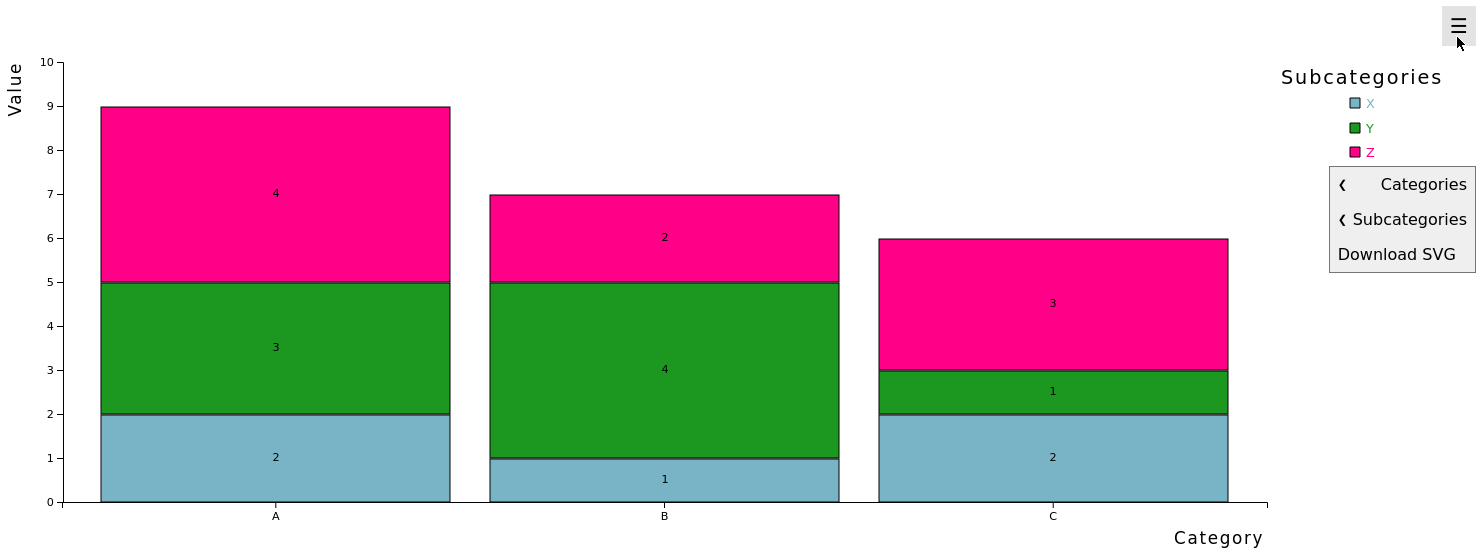
\includegraphics[keepaspectratio,width=\linewidth,height=\fullh]{images/stacked-bar-chart-window.png}
\hspace{1cm}
\label{fig:StackedBarChartWindow1}
}
\hspace{1cm}
\subfloat[Percent Stacked Bar Chart]{%
\hspace{1cm}
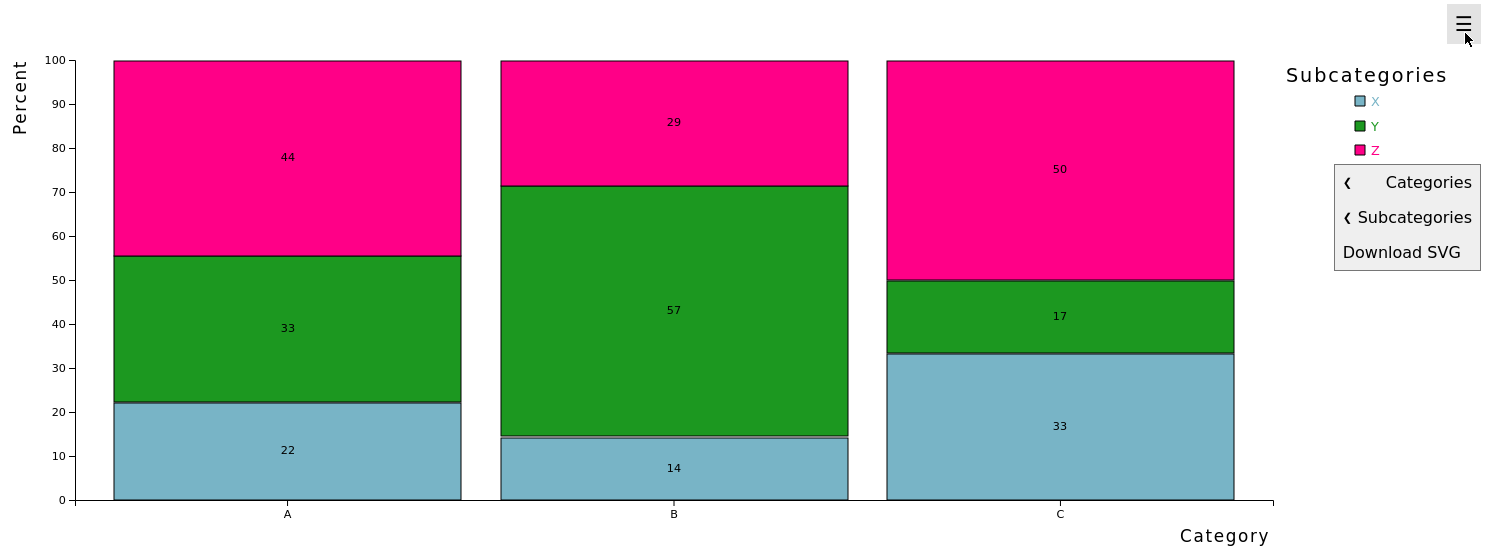
\includegraphics[keepaspectratio,width=\linewidth,height=\fullh]{images/percent-stacked-bar-chart-window.png}
\hspace{1cm}
\label{fig:StackedBarChartWindow2}
}
\caption[Stacked Bar Chart Window Example]{%
  The resulting Stacked Bar Charts of the example code in Listing~\ref{list:StackedBarChartWindow}. 
  The tool menu popup has manually been displaced to not cover the legend.
  \subref{fig:StackedBarChartWindow1} A Basic Stacked Bar Chart to compare the category totals and subcategory contributions to these totals.
  \subref{fig:StackedBarChartWindow2} A Percent Stacked Bar Chart to better compare the subcategory contributions to category totals. 
  \imgcredit{Image created by the author of this thesis using RespVis.}
}
\label{fig:StackedBarChartWindow}
\end{figure}
  


\section{Point Module}

Point Charts, manchmal auch scatter charts oder scatter plots genannt, werden verwendet um die beziehung zwischen zwei dimensionen eines datensatzes ueber punkte in einem kartesischen koordinatensystem zu verdeutlichen.
ueber eine solche visualisierung koennen potentielle korrelationen und muster zwischen diesen dimensionen identifiziert werden.
ueblicherweise werden zwei numerische dimensionen fuer die positionierung der punkte verwendet.
die art der zu visualisierenden daten ist jedoch nicht von bedeutung, solange individuelle werte ueber eine scale auf raeumliche dimensionen abgebildet werden koennen.
durch zusaetzliche kodierung der punkte mit farben, groessen oder formen koennen mehr als zwei dimensionen in einem Point Chart visualisiert werden.
Point Charts in welchen eine dritte dimension ueber die groesse der punkte visualisiert wird, werden auch bubble charts genannt.
der source code um einen skalierenden Point Chart mit der RespVis library zu erzeugen befindet sich in Listing~\ref{list:PointChartWindow} und die daraus resultierende visualisierung kann in Figure~\ref{fig:PointChartWindow} gesehen werden.  

\begin{samepage}
\lstinputlisting[%
  float=tp,
  aboveskip=\floatsep,
  belowskip=\floatsep,
  xleftmargin=0cm,              % no extra margins for floats
  xrightmargin=0cm,             % no extra margins for floats
  %
  basicstyle=\footnotesize\ttfamily,
  frame=shadowbox,
  numbers=left,
  label=list:PointChartWindow,
  caption={[Point Chart Window Example]%
    The example source code that creates a Point Chart Window.
    The Point Chart Window is configured with a bound data object that is initialized via the \code{chartWindowPointData} function.
    After configuration, the Chart Window is rendered by the \code{chartWindowPointRender} function.
    Since no special responsive behavior is desired in this example, the default resize behavior is attached to the Chart Window via the \code{chartWindowPointAutoResize} function. 
  },
]{listings/point-chart-window.js}
\end{samepage}
  

\begin{figure}[tp]
\centering
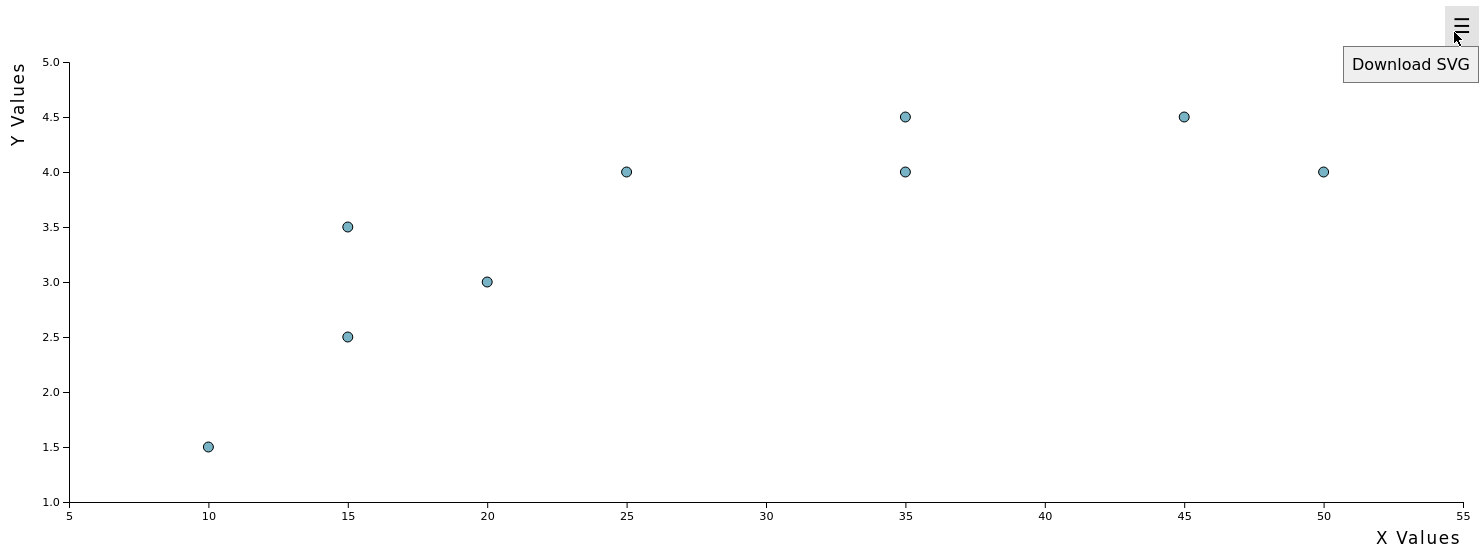
\includegraphics[keepaspectratio,width=\linewidth,height=\fullh]{images/point-chart-window.png}
\caption[Point Chart Window Example]{
  The resulting Point Chart of the example code in Listing~\ref{list:PointChartWindow}. 
  \imgcredit{Image created by the author of this thesis using RespVis.}
}
\label{fig:PointChartWindow}
\end{figure}
  

das Point Module befindet sich im \code{src/lib/point/} ordner der RespVis library und beinhaltet die implementierung der Point Series, Point Chart, und Point Chart Window komponenten.
mit einer Point Series wird eine sammlung an \code{<circle>} elementen gerendert deren mittelpunkte ueber X und Y werte arrays mit deren dazugehoerigen X und Y scales bestimmt werden und deren styles ueber style klassen gesetzt werden.
da die radiuse der einzelnen \code{<circle>} elemente konfigurierbar sind, kann eine Point Series auch verwendet werden um einen bubble chart zu erzeugen.
wie auch bei anderen Series Components, wird auch hier das gebundene datenobjekt in ein array an datenobjekten transformiert welches verwendet wird um die elemente der Series ueber einen data join zu rendern.
ein Point Chart ist ein kartesischer Chart mit einer Point Series in seiner draw area und zwei achsen welche die scales visualisieren mit welchen die Point Series gerendert wurde.
Point Chart Windows sind wrapper komponenten um Point Charts die diese in einen Layouter einbetten, ihren render prozess abwickeln, und sie mit einer toolbar dekorieren.
zum aktuellen zeitpunkt wird nur ein SVG download tool ueber die toolbar eines Point Chart Windows zur verfuegung gestellt da bislang nur eine begrenzte anzahl an tools entwickelt wurden und diese sich nicht fuer die anwendung an Point Charts eignen.
werden weitere tools benoetigt muessen diese manuell von visualisierungsauthoren implementiert und hinzugefuegt werden.